\usepackage{tikz}
\usetikzlibrary{arrows.meta, positioning, shapes.geometric, calc}

\section{Introduction}

Large language model (LLM) agents are rapidly moving from prototypes to production systems.
They now power customer support assistants, internal copilots, analytics dashboards, and workflow automations that call internal tools and APIs.
In these settings, an agent is not just ``a model'' but a \emph{service} that must satisfy explicit contracts and service-level objectives (SLOs): it must emit JSON or other structured outputs that downstream systems can parse, must stay faithful to the underlying data or retrieved context, and must respond within a bounded latency for an acceptable user experience.
If an agent emits malformed JSON, downstream ETL jobs or dashboards may fail.
If it emits a plausible but unsupported statement about a key metric, decision-makers may act on a hallucination.
If it is occasionally fast but has heavy-tailed latency, users perceive the system as unreliable and throughput collapses.

Systems research has long emphasized that users experience \emph{tail latency}, not averages.
Dean and Barroso's ``The Tail at Scale''~\citep{dean2013tail} (\url{https://cacm.acm.org/research/the-tail-at-scale/}) showed that even a small fraction of slow requests can dominate perceived quality and limit scalability.
Modern LLM-serving work extends this insight to Transformer inference.
Runtimes such as vLLM~\citep{kwon2023vllm} (\url{https://arxiv.org/abs/2309.06180}), SGLang~\citep{zheng2023sglang} (\url{https://arxiv.org/abs/2312.07104}), DeepSpeed-FastGen~\citep{deepspeedFastGen} (\url{https://arxiv.org/abs/2401.08671}), and Sarathi-Serve~\citep{agrawal2024sarathi} (\url{https://www.usenix.org/system/files/osdi24-agrawal.pdf}) propose kernel and scheduling optimizations---paged KV caches, optimized attention kernels~\citep{dao2023flashattention2,prabhu2024vattention}, speculative decoding~\citep{leviathan2023speculative} (\url{https://arxiv.org/abs/2211.17192})---that improve throughput and reduce tail latency.
However, these systems generally treat the model as a black box that emits free-form text and do not reason explicitly about structured contracts or the \emph{semantic} correctness and faithfulness of responses.

In parallel, API providers and local runtimes have introduced \emph{structured output} modes.
OpenAI's structured outputs and function-calling interfaces (\url{https://openai.com/index/introducing-structured-outputs-in-the-api/}), Azure OpenAI, and Snowflake Cortex (\url{https://docs.snowflake.com/en/user-guide/snowflake-cortex/complete-structured-outputs}) expose JSON Schema-like contracts that models are expected to obey.
Local stacks such as LM Studio (\url{https://lmstudio.ai/docs/developer/openai-compat/tools}) and Ollama (\url{https://docs.ollama.com/capabilities/structured-outputs}, \url{https://blog.danielclayton.co.uk/posts/ollama-structured-outputs/}) provide OpenAI-compatible endpoints with structured-output options.
Libraries like Outlines (\url{https://dottxt-ai.github.io/outlines/}), Instructor (\url{https://python.useinstructor.com/integrations/llama-cpp-python/}), and llama.cpp grammars (\url{https://github.com/ggml-org/llama.cpp/blob/master/grammars/README.md}) compile contracts into grammars or JSON constraints.
Recent benchmarks such as JSONSchemaBench and analyses of format constraints~\citep{geng2025jsonschemabench,letmespeakfreely,structuredRAG} (\url{https://arxiv.org/abs/2501.10868}, \url{https://arxiv.org/abs/2408.02442}, \url{https://arxiv.org/abs/2408.11061}) show that constrained decoding substantially improves syntactic validity.
Yet these works leave open how structured decoding interacts with serving runtimes, tail latency, and business-level metrics such as task success and SLO adherence.

Beyond format, \emph{faithfulness}---whether an agent's output is supported by the underlying data or retrieved context---has emerged as a central concern.
For many commercial agents, the primary risk is not that the model produces ungrammatical text, but that it produces fluent, confident statements that are subtly wrong.
RAGAS (Retrieval Augmented Generation Assessment)~\citep{es2023ragas} (\url{https://arxiv.org/abs/2309.15217}) proposed automated metrics for retrieval-augmented generation (RAG) that use an LLM judge to score faithfulness and answer relevance.
Subsequent work on ``atomic fact'' evaluation~\citep{atomicFacts2024} (\url{https://arxiv.org/abs/2408.15171}) advocates decomposing responses into fine-grained statements and checking each against the context to better characterize hallucinations.
These approaches, however, are mostly experimental and are not tightly tied to structured outputs that feed downstream systems or to latency-aware SLOs.

Cloud providers and tooling ecosystems have started to articulate evaluation methods for agents in production.
Google's Agent Development Kit (ADK) and Vertex AI evaluation documentation (\url{https://google.github.io/adk-docs/evaluate/}, \url{https://cloud.google.com/vertex-ai/generative-ai/docs/models/evaluation-overview}) emphasize evaluating both final response quality and \emph{trajectory} quality (tools invoked, step counts, error handling) using golden sets and task-specific rubrics.
Google Cloud's blogs on agent testing and evaluation (\url{https://medium.com/google-cloud/agent-testing-and-evaluation-methods-64d1bd9ac44f}, \url{https://cloud.google.com/blog/topics/developers-practitioners/a-methodical-approach-to-agent-evaluation/}) and the LLM-Evalkit tools (\url{https://github.com/GoogleCloudPlatform/generative-ai/tree/main/tools/llmevalkit}, \url{https://cloud.google.com/blog/products/ai-machine-learning/introducing-llm-evalkit}) offer practical recipes for building evaluation pipelines.
These resources are valuable, but they are high-level and platform-specific: they do not define a concrete, portable test suite that ties together structured outputs, faithfulness metrics, trajectory checks, and tail-latency SLOs for agents running on local backends such as LM Studio, Ollama, or vLLM.

In this work we focus on the regime where a team runs a \emph{single-GPU} agent stack---for example, an RTX 4090 in an on-premise box or a MacBook Pro with Apple Silicon---and serves generic agents via local OpenAI-compatible servers (e.g., LM Studio: \url{https://lmstudio.ai/docs/developer/openai-compat/tools}; Ollama: \url{https://docs.ollama.com/capabilities/structured-outputs}; vLLM: \url{https://arxiv.org/abs/2309.06180}).
The agents must emit structured JSON outputs that downstream systems can consume, remain faithful to internal data or retrieved context, and respect p95/p99 latency budgets, all under tight compute and privacy constraints.
Practically, this scenario is common: teams want to avoid sending sensitive data to external APIs, want predictable costs, and still need high-quality agent behavior.
Crucially, in many of these use cases, \emph{correctness and truthfulness are prioritized over speed}, except where a specific real-time SLA explicitly dominates.

We argue that what is missing is a \textbf{contract-first, SLO-aware agent framework} that:
(i) treats JSON Schemas and grammars as the primary interface between applications and LLMs;
(ii) assesses not only syntactic validity but also task accuracy, statement-level faithfulness, tool and trajectory behavior, stability across runs, and SLO adherence; and
(iii) is designed to run on single-GPU local backends rather than assuming large managed clusters.
Such a framework should support both \emph{static evaluation} of a given policy and configuration and \emph{dynamic improvement} via reinforcement learning, so that agents can become more reliable over time while staying within latency and cost envelopes.

We make three contributions toward this goal:
\begin{itemize}[leftmargin=12pt]
    \item \textbf{A contract-first, single-GPU agent architecture.}
    We introduce a spec-driven agent architecture that treats JSON Schemas and grammars as first-class contracts, compiles them into structured decoding for LM Studio, Ollama, vLLM, and llama.cpp, and integrates bounded validation-and-retry and budgeted self-consistency under explicit wall-clock and token budgets on a single GPU.
    \item \textbf{A unified, configurable evaluation suite for agents.}
    We design an auditable evaluation framework, configured via a single \texttt{criteria.yaml}, that spans six metric families---structure, task accuracy, faithfulness, tools and trajectories, stability, and latency/SLOs---and can be applied unchanged across backends and models.
    The framework organizes a 100+ test suite, logs all runs to Weights \& Biases (W\&B) for reproducibility (\url{https://docs.wandb.ai/models/quickstart}, \url{https://docs.wandb.ai/models/artifacts}, \url{https://docs.wandb.ai/models/evaluate-models}), and is designed to capture real-world failure modes that matter to practitioners.
    \item \textbf{A measurement study of decoding modes and backends under SLOs.}
    We provide a measurement study on RTX 4090 and M2 Max that compares unconstrained decoding, provider-native structured outputs, grammar-based constraints, and our full spec-driven approach across LM Studio, Ollama, and vLLM.
    We show how these modes reshape the trade-off frontier between structural correctness, faithfulness, Success@\slo, and tail latency, and we illustrate how the same metrics can be reused as reward components and constraints in single-GPU TRL PPO/GRPO loops~\citep{schulman2017ppo,grpo,dettmers2023qlora} (\url{https://huggingface.co/docs/trl/en/logging}, \url{https://huggingface.co/docs/trl/en/grpo_trainer}).
\end{itemize}

The remainder of this paper is organized as follows.
Section~\ref{sec:background} reviews related work in LLM serving, structured decoding, and agent evaluation.
Section~\ref{sec:problem} formulates contract-first, SLO-aware agent serving as a constrained optimization problem.
Section~\ref{sec:method} describes our spec-to-decoder compilation, validation-and-retry, budgeted self-consistency, and single-GPU serving design.
Section~\ref{sec:eval-framework} presents the evaluation framework and test families in detail, including our faithfulness scorer and trajectory tests.
Section~\ref{sec:experiments} reports single-GPU experiments and a measurement study of decoding modes and backends.
Section~\ref{sec:discussion} discusses limitations and future directions, including safety, multi-turn interactions, and deeper RL integration.

\section{Background and Related Work}
\label{sec:background}

Our work sits at the intersection of systems for LLM serving, structured decoding and contract-first generation, automated evaluation of faithfulness and reliability, and emerging agent evaluation frameworks used in production environments.
This section reviews prior work in each of these areas and highlights the gaps that SpecSLOEval is designed to fill.

\subsection{Tail Latency and LLM Serving}

Classic systems work emphasizes that users experience the worst-case behavior of a service rather than its average latency.
Dean and Barroso's ``The Tail at Scale''~\citep{dean2013tail} (\url{https://cacm.acm.org/research/the-tail-at-scale/}) shows that even a small fraction of slow requests can dominate perceived quality and limit system scalability.
They advocate design principles that explicitly target tail latency---\pninetyfive, \pninetynine---through redundancy, hedging, careful queueing, and resource management.

LLM-serving work inherits these concerns and exacerbates them due to high per-request compute costs, variable-length outputs, and complex batching behavior.
vLLM introduces PagedAttention to provide efficient KV-cache management and continuous batching, significantly improving throughput and memory utilization for transformer models~\citep{kwon2023vllm} (\url{https://arxiv.org/abs/2309.06180}).
SGLang focuses on efficient execution of structured language model programs, proposing system-level optimizations such as speculative execution of subprograms and optimized scheduling~\citep{zheng2023sglang} (\url{https://arxiv.org/abs/2312.07104}).
DeepSpeed-FastGen~\citep{deepspeedFastGen} (\url{https://arxiv.org/abs/2401.08671}) and vAttention~\citep{prabhu2024vattention} (\url{https://arxiv.org/abs/2405.04437}) introduce kernel and memory-layout optimizations that reduce compute and memory overhead, further helping tail latency.
FlashAttention-2~\citep{dao2023flashattention2} (\url{https://arxiv.org/abs/2307.08691}) redesigns the attention kernel for better parallelism and cache usage.
Speculative decoding, as described by Leviathan \etal~\citep{leviathan2023speculative} (\url{https://arxiv.org/abs/2211.17192}), drafts tokens with a smaller model and verifies them with the target model to reduce time-to-first-token.

Sarathi-Serve~\citep{agrawal2024sarathi} (\url{https://www.usenix.org/system/files/osdi24-agrawal.pdf}) takes a holistic view of throughput-latency trade-offs for LLM inference, examining queueing models and scheduling policies under realistic traffic patterns and mixed workloads.
However, these systems papers generally treat the model as a black box that emits unconstrained text and focus on hardware and scheduling.
They do not reason about the \emph{structure} or \emph{semantics} of outputs (e.g., JSON validity, schema adherence, faithfulness to context), and they typically assume multi-GPU clusters or cloud-scale deployments rather than single-GPU setups.

By contrast, our focus is on single-GPU serving (RTX~4090 or equivalent, Apple M-series) for agents that must satisfy contracts and SLOs.
We build on the scheduling and kernel-level insights from vLLM, Sarathi-Serve, DeepSpeed-FastGen, and related work, but integrate them with contract-first decoding and a multi-metric evaluation suite tailored to structured agent use cases.
SpecSLOEval is concerned not only with how \emph{fast} agents produce text, but also with whether that text is structurally valid, faithful, stable, and compatible with downstream systems.

\subsection{Structured Outputs, Grammars, and Contract-First Decoding}

Many real-world applications want structured outputs—JSON documents, typed objects, or tool-call payloads—not arbitrary free-form text.
API providers have responded with structured-output modes.
OpenAI introduced function calling and structured outputs (\url{https://openai.com/index/introducing-structured-outputs-in-the-api/}), which allow developers to specify JSON Schema-like contracts that the model is expected to satisfy.
Azure OpenAI and Snowflake Cortex provide similar capabilities for structured completions and strongly typed outputs (\url{https://docs.snowflake.com/en/user-guide/snowflake-cortex/complete-structured-outputs}).

Local runtimes mirror these trends.
LM Studio exposes an OpenAI-compatible interface for local models, including tools and structured outputs (\url{https://lmstudio.ai/docs/developer/openai-compat/tools}).
Ollama provides structured-output capabilities and supporting documentation (\url{https://docs.ollama.com/capabilities/structured-outputs}, \url{https://blog.danielclayton.co.uk/posts/ollama-structured-outputs/}).
Fireworks.ai advocates for structured output modes across all LLMs, emphasizing reductions in integration errors and easier downstream processing (\url{https://fireworks.ai/blog/why-do-all-LLMs-need-structured-output-modes}).

Beyond provider-specific APIs, open-source libraries and runtimes support generic contract-first tooling.
Outlines~\citep{outlinesDocs} (\url{https://dottxt-ai.github.io/outlines/}) implements grammar-based decoding for regular languages and JSON, enforcing Pydantic models on top of arbitrary providers.
`llama.cpp` supports GBNF grammars (\url{https://github.com/ggml-org/llama.cpp/blob/master/grammars/README.md}), enabling constrained decoding even with local C++ inference.
Instructor (\url{https://python.useinstructor.com/integrations/llama-cpp-python/}) layers structured decoding on `llama-cpp-python` and constructs typed Python objects from LLM outputs.

Recent benchmark efforts explicitly investigate structured generation.
JSONSchemaBench~\citep{geng2025jsonschemabench} (\url{https://arxiv.org/abs/2501.10868}) proposes standardized JSON Schema tasks to test the ability of LLMs to follow structured contracts.
Studies of format constraints and structured RAG~\citep{letmespeakfreely,structuredRAG} (\url{https://arxiv.org/abs/2408.02442}, \url{https://arxiv.org/abs/2408.11061}) show that forcing specific formats can improve syntactic validity but may interact with other output properties (e.g., verbosity, creativity, over-constraining content).

These works collectively show that structured decoding is powerful and that contracts can be compiled into provider- and runtime-specific constraints.
However, they primarily evaluate contract adherence in isolation: does the model produce syntactically valid JSON given a schema?
They do not systematically study how structured decoding interacts with:
(i) serving runtimes and tail latency;
(ii) multi-dimensional evaluation metrics (faithfulness, stability, tool behavior, SLOs); or
(iii) single-GPU local deployment constraints.

SpecSLOEval treats structured decoding as one layer in a larger agent stack.
We define contracts once, compile them into backends such as LM Studio, vLLM, and llama.cpp, and connect them to an evaluation framework that measures not only schema adherence but also task accuracy, faithfulness, trajectories, stability, and SLO adherence in realistic agent workflows.

\subsection{Automated Evaluation of Faithfulness and Factuality}

Evaluating the faithfulness or factuality of LLM outputs is challenging, particularly when ground truth is complex or implicit.
RAGAS (Retrieval Augmented Generation Assessment)~\citep{es2023ragas} (\url{https://arxiv.org/abs/2309.15217}) proposes automatic metrics for retrieval-augmented generation, including \emph{faithfulness} (does the answer contradict the context?) and \emph{answer correctness}.
RAGAS typically uses an LLM-as-judge setup: a judge model receives the context and the answer and assigns scores.
This design has influenced many RAG evaluation pipelines in industry and open-source tooling.

Other work advocates decomposing responses into ``atomic facts'' and scoring each fact separately, improving interpretability and reducing the risk that a single aggregate score hides critical errors.
Kriman \etal~\citep{atomicFacts2024} (\url{https://arxiv.org/abs/2408.15171}) propose atomic-fact–based evaluation for summarization, extracting fine-grained claims and checking each against the source.
This style of evaluation is particularly relevant for agents that summarize logs, documents, or metrics: a short narrative can be decomposed into claims such as ``metric X increased week-over-week'' or ``customer Y is in segment Z'', each of which can be checked against data.

At the same time, several studies warn that LLM-as-judge setups can be biased and unstable.
For example, recent work on LLM judges~\citep{llmjudgebias} (\url{https://arxiv.org/abs/2305.17926}) documents positional bias, sensitivity to phrasing, and preferences for verbose answers, raising concerns about using LLMs as the sole evaluators in high-stakes contexts.
This motivates treating judge-based metrics as proxies that must be calibrated and complemented with other signals.

Our framework adopts the insights of RAGAS and atomic-fact evaluation but adapts them to structured agent outputs and SLO-constrained settings.
We:
(i) restrict attention to contexts where ground truth support is relatively clear (e.g., numeric or tabular data, concrete documents);
(ii) use a 0--3 support scale with an explicit contradiction flag, increasing granularity;
(iii) calibrate thresholds with small human-labeled subsets; and
(iv) treat the judge-based faithfulness metric as one component of a broader metric vector, not a standalone arbiter.
SpecSLOEval is designed so that faithfulness signals can be used both for static assessment and as reward components in RL, while acknowledging the limitations of judge models.

\subsection{Agent Evaluation Frameworks in Practice}

Cloud providers and tool vendors have begun to systematize agent evaluation, especially for tool-using and workflow-oriented agents.
Google's Agent Development Kit (ADK) documentation on ``Why Evaluate Agents'' (\url{https://google.github.io/adk-docs/evaluate/}) argues that agents should be evaluated both on final response quality and on the quality of trajectories (tool choices, sequencing, error handling).
Google Cloud's blog posts on agent testing and evaluation (\url{https://medium.com/google-cloud/agent-testing-and-evaluation-methods-64d1bd9ac44f}, \url{https://cloud.google.com/blog/topics/developers-practitioners/a-methodical-approach-to-agent-evaluation/}) recommend golden sets, task-specific rubrics, and coverage-oriented testing.
Vertex AI's evaluation overview (\url{https://cloud.google.com/vertex-ai/generative-ai/docs/models/evaluation-overview}) and the LLM-Evalkit tools (\url{https://github.com/GoogleCloudPlatform/generative-ai/tree/main/tools/llmevalkit}, \url{https://cloud.google.com/blog/products/ai-machine-learning/introducing-llm-evalkit}) provide code templates and metrics for evaluating Vertex-hosted models and agents.

These resources establish useful concepts---golden datasets, agent ``unit tests,'' trajectory inspection—but they are tied to specific cloud platforms and assumptions about where the model is hosted.
They typically focus on final answer quality, simple success flags, or coarse-grained business metrics, and leave structural, faithfulness, stability, and SLO-specific metrics under-specified.
Moreover, they do not directly address agents running on local, single-GPU backends such as LM Studio or Ollama, where privacy and cost constraints differ from cloud settings.

SpecSLOEval generalizes these practices by:
(i) defining a backend-agnostic test suite, expressed declaratively in a single \texttt{criteria.yaml}, that can be executed against local or cloud-hosted endpoints;
(ii) making structure, task accuracy, faithfulness, tools/trajectories, stability, and SLOs first-class metric families; and
(iii) integrating evaluation outputs with CI and RL pipelines via W\&B logging (\url{https://docs.wandb.ai/models/quickstart}, \url{https://docs.wandb.ai/models/artifacts}, \url{https://docs.wandb.ai/models/evaluate-models}).
This adds a concrete, portable realization of ideas that cloud evaluation docs describe at a higher level.

\subsection{Single-GPU Local Serving and Open-Weight Models}

A key practical difference between many academic systems papers and our target environment is the hardware and deployment model.
Instead of assuming multi-GPU clusters or managed APIs, we explicitly target \emph{single-node} deployments: a workstation with an RTX~4090 or a laptop-class device with Apple M-series, running local OpenAI-compatible servers.

LM Studio documentation describes how to run local endpoints and load open-weight models via an OpenAI-compatible interface (\url{https://lmstudio.ai/docs/developer/openai-compat/tools}, \url{https://lmstudio.ai/models}).
Qwen's documentation explains how to host Qwen models locally and via OpenAI-like APIs (\url{https://qwen.readthedocs.io/en/latest/getting_started/quickstart.html}).
Ollama offers a simple CLI and HTTP API for running models locally with optional structured outputs (\url{https://docs.ollama.com/capabilities/structured-outputs}).
vLLM is frequently used as a high-performance backend for open-weight models, with recipes for deployment on services like Modal~\citep{kwon2023vllm} (\url{https://modal.com/docs/examples/vllm_inference}).
llama.cpp provides highly optimized CPU/GPU inference for quantized models.

These tools make it possible for small teams to run reasonably capable LLM agents entirely on their own hardware, but they do not dictate how agents should be evaluated, how contracts should be enforced, or how SLOs should be defined.
SpecSLOEval is designed to sit above these runtimes: it assumes only an OpenAI-compatible API and sufficient observability (latency, token counts, prompts, responses) to compute metrics and log them to W\&B.
By focusing on single-GPU local serving for structured agents, we bridge a gap between large-scale, research-oriented serving work and the needs of teams that want to deploy agents securely and predictably on their own infrastructure.

This background motivates our problem formulation.
In the next section, we formalize contract-first, SLO-aware agent serving as a constrained optimization problem and introduce the metric families and configuration surface that underpin SpecSLOEval.

\section{Problem Formulation}
\label{sec:problem}

Figure~\ref{fig:agent-context} sketches the setting we target.
A generic commercial agent sits between upstream requesters (users, batch jobs, or other services) and downstream consumers (dashboards, workflows, humans).
For each request, the agent receives unstructured and structured context (documents, logs, records, prior turns), may call tools (APIs, databases, services), and is expected to emit \emph{structured outputs} such as JSON reports, action recommendations, or tool-call payloads.
These outputs do not only surface in a chat window; they are consumed by campaign engines, scoring pipelines, ETL jobs, monitoring dashboards, and human decision-makers.
Small model errors can therefore propagate and compound:
a malformed JSON object may crash a downstream job;
a mis-typed field can poison an aggregate;
a subtly incorrect statement about a key metric may trigger the wrong business action.
At the same time, users and systems experience the agent through latency: if responses frequently violate p95/p99 latency budgets, trust erodes even when mean latency and accuracy look acceptable.

We want a formulation that is:
(i) amenable to systems-level analysis (latency distributions, SLO constraints, single-GPU capacity);
(ii) fine-grained enough to capture semantics (structure, task accuracy, faithfulness, tool behavior, stability);
and (iii) compatible with both static evaluation and reinforcement-learning-based improvement.
We therefore define:
an abstract \emph{agent and contract model} (Section~\ref{sec:problem-agent}),
a \emph{serving environment} with explicit latency-based SLOs (Section~\ref{sec:problem-slo}),
and a vector of \emph{evaluation metrics} configured via a single criteria file (Section~\ref{sec:problem-metrics}).
Figure~\ref{fig:metric-families} summarizes the metric families; Figure~\ref{fig:optimization-view} gives an optimization view that supports both static configuration search and constrained RL.

Throughout this section we use the term \emph{configuration} for a concrete choice of model, runtime, decoding settings, and contract.
The rest of the paper instantiates this formulation for single-GPU deployments (RTX~4090 or Apple M-series) and a standard set of evaluation tasks.

\subsection{Agent, Contract, and Configuration}
\label{sec:problem-agent}

We formalize an \emph{agent invocation} as a single request--response episode.
Let $\mathcal{X}$ denote the space of requests.
Each request $x \in \mathcal{X}$ may consist of:
\begin{itemize}[leftmargin=12pt]
    \item a user instruction or task description (free-form text or a structured spec),
    \item a multiset of context items $C = \{c_1,\dots,c_m\}$ such as retrieved documents, KB entries, prior turns, log excerpts, or database records,
    \item optional metadata such as user profile, locale, device information, or authorization context.
\end{itemize}
We deliberately keep $\mathcal{X}$ domain-agnostic: the same formalism covers analytics summarization, support automation, code editing, incident response, and other agent tasks.

For each request $x$, the agent must produce one or more outputs $y$ in an output space $\mathcal{Y}$.
The structure of $\mathcal{Y}$ is governed by a \emph{contract} $\mathcal{C}$.
In practical systems, such contracts are written as JSON Schemas, Pydantic models, protocol buffer definitions, or grammars.
We abstract this as a predicate
\[
\mathcal{C} : \mathcal{Y} \to \{0,1\},
\]
which returns $1$ if and only if $y$ is syntactically well formed (e.g., valid JSON) and satisfies all structural constraints:
field presence, types, enum values, bounds, nesting, and any additional invariants encoded in the contract (e.g., fields that must sum to one, monotonicity constraints).
By \emph{contract-first} we mean that $\mathcal{C}$ is specified before the agent is invoked and that decoding is explicitly designed to respect $\mathcal{C}$ rather than being retrofitted after the fact.

We assume a parametric policy $\pi_\theta$, typically an LLM with prompts and optionally fine-tuned weights or adapters.
The policy is deployed via a serving runtime $R$ (e.g., LM Studio, Ollama, vLLM, or \texttt{llama.cpp}) that exposes an OpenAI-compatible API.
Given a request $x$, contract $\mathcal{C}$, and decoding configuration $\delta$ (temperature, top-$p$, maximum tokens, number of self-consistency samples $k$, batch size, speculative-decoding flags, etc.), the agent induces a conditional distribution over outputs
\[
y \sim \pi_\theta(\cdot \mid x, \mathcal{C}, \delta, R).
\]

Modern runtimes support different mechanisms to enforce or approximate the contract $\mathcal{C}$:
\begin{itemize}[leftmargin=12pt]
    \item \textbf{Provider-native constraints.}
    Here $\mathcal{C}$ is translated into a schema or tool spec understood directly by the serving runtime.
    Examples include OpenAI-style \texttt{response\_format} and function calling (\url{https://openai.com/index/introducing-structured-outputs-in-the-api/}), LM Studio’s OpenAI-compatible tools (\url{https://lmstudio.ai/docs/developer/openai-compat/tools}), and Ollama’s structured outputs (\url{https://docs.ollama.com/capabilities/structured-outputs}).
    \item \textbf{Library-based or post-hoc constraints.}
    Here $\mathcal{C}$ is enforced via third-party libraries and explicit validation-and-retry logic.
    Examples include Outlines (\url{https://dottxt-ai.github.io/outlines/}) and GBNF grammars in \texttt{llama.cpp} (\url{https://github.com/ggml-org/llama.cpp/blob/master/grammars/README.md}), combined with JSON schema validation libraries.
\end{itemize}
From the agent’s perspective, the contract $\mathcal{C}$ and the configuration $\delta$ are part of its \emph{effective policy}: changing either alters the mapping $x \mapsto y$ even if the underlying model weights remain fixed.

For compactness, we write a \emph{configuration} as
\[
\kappa = (R,\pi_\theta,\delta,\mathcal{C}).
\]
Given a workload (distribution over requests) $W$ and environment (tools, data sources), a configuration $\kappa$ induces a distribution over episodes and outputs.
The goal of our framework is to evaluate and ultimately optimize over such configurations under realistic workload and SLO constraints.

\subsection{Serving Environment and Latency SLOs}
\label{sec:problem-slo}

We assume the agent stack runs on a \emph{single, finite-capacity node} equipped with a GPU (e.g., NVIDIA RTX~4090) or a laptop-class accelerator (e.g., Apple M2 Max).
The serving runtime $R$ performs prefill and decoding, possibly batching multiple requests, managing KV caches, and using techniques such as PagedAttention as in vLLM~\citep{kwon2023vllm} (\url{https://arxiv.org/abs/2309.06180}).

For each request $x$ served under configuration $\kappa$, we define the end-to-end latency
\[
L_\kappa(x) = t_{\text{finish}}(x) - t_{\text{start}}(x),
\]
where $t_{\text{start}}(x)$ is the time when $x$ is submitted to the serving system and $t_{\text{finish}}(x)$ is the time when a fully validated structured output $y$ (or an explicit error) is available to downstream consumers.
By “fully validated” we mean that validation-and-retry logic has run, contracts have been checked, and any fallback behavior has completed.

Requests arrive according to a stochastic workload model that may include bursts, diurnal patterns, and varying context sizes.
We denote this workload model by $W$, which induces both a sequence of arrival times and a distribution over request payloads $x \in \mathcal{X}$.
Given $\kappa$ and $W$, the induced latency distribution is
\[
Q_\kappa^W = \mathcal{L}\big(L_\kappa(x) \mid x \sim W\big),
\]
and we summarize it via quantiles
\[
\mathrm{p50}(Q_\kappa^W),\quad \mathrm{p95}(Q_\kappa^W),\quad \mathrm{p99}(Q_\kappa^W),
\]
and, when relevant, time-to-first-token (TTFT) and throughput (queries per second, QPS).
Following \citet{dean2013tail}, \pninetyfive and \pninetynine are treated as first-class metrics: they control perceived responsiveness and throughput in multi-step, fan-out-heavy systems.

Service-level objectives (\slo s) are typically expressed as bounds on these quantiles.
A common pattern is:
\[
\mathrm{p95}(Q_\kappa^W) \leq B,\qquad \mathrm{p99}(Q_\kappa^W) \leq B',
\]
for budgets $B$ and $B'$ in milliseconds (e.g., 800~ms and 2000~ms).
Some organizations also specify hard timeouts (e.g., “no request may exceed 5 seconds”) or constraints on TTFT (e.g., “TTFT must be below 300~ms for chat experiences”).

Critically, in many enterprise settings latency is not the \emph{primary} objective.
Stakeholders often adopt a \emph{lexicographic} preference ordering:
\begin{itemize}[leftmargin=12pt]
    \item \textbf{First, correctness and structure.}
    Outputs must be structurally valid (JSON parses and satisfies $\mathcal{C}$) and semantically correct (task accuracy and faithfulness above thresholds).
    A fast but hallucinated or malformed response is worse than a slower but correct one.
    \item \textbf{Second, stability.}
    Given correctness, outputs should be stable across seeds, versions, and days.
    Large unexplained fluctuations erode user trust and complicate monitoring.
    \item \textbf{Third, latency.}
    Given correctness and stability, latency should satisfy agreed SLOs.
    Only in explicitly latency-dominant applications (e.g., real-time trading, user-typing completions) does speed dominate correctness.
\end{itemize}
We encode this preference in our evaluation criteria and reward design: latency appears primarily as a \emph{constraint} and only secondarily as a negatively weighted objective, except for configurations explicitly marked as speed-critical.

To capture the combined notion of “correct and fast enough,” we define an episode-level indicator
\[
\text{Success@\slo}_\kappa(x) =
\begin{cases}
1 & \text{if the episode satisfies all selected quality criteria and latency constraints},\\[2pt]
0 & \text{otherwise.}
\end{cases}
\]
Quality criteria are derived from the metric vector $m_\kappa(x,y)$ (Section~\ref{sec:problem-metrics}); latency constraints are derived from $Q_\kappa^W$ and budgets $(B,B')$.
Aggregating Success@\slo over an evaluation set yields a concise, business-aligned metric: the fraction of requests that are both \emph{good} and \emph{on time}.

\subsection{Metric Families and Criteria Configuration}
\label{sec:problem-metrics}

To reason about agents in a way that is auditable, tunable, and reusable across backends, we define for each episode a metric vector
\[
m_\kappa(x,y) \in \mathbb{R}^K,
\]
whose components are grouped into families as illustrated in Figure~\ref{fig:metric-families}:
\emph{structure}, \emph{task accuracy}, \emph{faithfulness}, \emph{tools and trajectory}, \emph{stability}, and \emph{latency/SLOs}.
We briefly describe each here; Section~\ref{sec:eval-framework} gives concrete definitions and example tests.

\paragraph{Structure.}
Structural metrics capture whether the output is syntactically and contractually well formed:
\begin{itemize}[leftmargin=12pt]
    \item JSON parse success (binary: parses or not),
    \item schema validity under $\mathcal{C}$ (binary),
    \item detailed error codes (missing fields, extra fields, type mismatches, constraint violations).
\end{itemize}
These are necessary conditions for safe downstream consumption.
We log fine-grained error counts (e.g., per-field violation rates) for debugging and potential RL shaping, even if only coarse indicators feed primary scores.

\paragraph{Task accuracy.}
When ground-truth labels or references exist, we compute:
\begin{itemize}[leftmargin=12pt]
    \item macro- or micro-F1 for extraction and classification tasks,
    \item exact match (EM) or accuracy for QA-style tasks,
    \item pass@$k$ for code or function synthesis tasks.
\end{itemize}
These metrics answer the question “does the agent actually solve the task it was asked to solve?”, independently of style or latency.

\paragraph{Faithfulness.}
Faithfulness metrics quantify whether $y$ is supported by the context $C$.
Following RAGAS~\citep{es2023ragas} (\url{https://arxiv.org/abs/2309.15217}) and atomic-fact evaluation~\citep{atomicFacts2024} (\url{https://arxiv.org/abs/2408.15171}), we:
\begin{enumerate}[leftmargin=12pt]
    \item use a judge model to decompose $y$ into atomic statements;
    \item assign each statement a support score $s \in \{0,1,2,3\}$ (“not supported” to “strongly supported”) and a contradiction flag;
    \item aggregate these into a scalar $m_{\text{faith}}(x,y) \in [0,1]$ that reflects the fraction of strongly supported statements, the average support, and a penalty for contradictions.
\end{enumerate}
We treat faithfulness as distinct from task accuracy: an answer can match a label but still misrepresent or over-claim relative to the underlying evidence.

\paragraph{Tools and trajectories.}
For tool-using agents we log, per episode:
\begin{itemize}[leftmargin=12pt]
    \item tool-call success rates (valid arguments, no schema violations, non-error responses),
    \item trajectory statistics: number of tool calls, invalid-argument retries, redundant calls,
    \item deviation from expected plans when such plans exist (e.g., edit distance between expected and realized tool sequences), in the spirit of Google’s ADK (\url{https://google.github.io/adk-docs/evaluate/}) and LLM-Evalkit (\url{https://github.com/GoogleCloudPlatform/generative-ai/tree/main/tools/llmevalkit}).
\end{itemize}
These metrics expose how the agent behaves in the environment, not just what final JSON it produces.

\paragraph{Stability.}
Stability metrics quantify variability across runs:
\begin{itemize}[leftmargin=12pt]
    \item Disagreement@$k$, defined as one minus the fraction of “equivalent” outputs across $k$ repeated runs (where equivalence can be defined via schema-respecting canonicalization or atomic-fact overlap),
    \item variance of key metrics (e.g., accuracy, faithfulness) across random seeds, in line with recent work on LLM stability~\citep{llmStability} (\url{https://arxiv.org/abs/2408.04667}).
\end{itemize}
High instability—even at similar averages—can be operationally unacceptable.

\paragraph{Latency and SLOs.}
For each episode we record $L_\kappa(x)$ and, when relevant, TTFT.
Over an evaluation set $\mathcal{D}_{\text{eval}}$, we compute:
\begin{itemize}[leftmargin=12pt]
    \item p50, \pninetyfive, \pninetynine;
    \item Success@\slo rates under various budgets;
    \item tail-violation rates (fraction of requests exceeding hard cutoffs).
\end{itemize}
These metrics capture responsiveness and capacity under the chosen configuration.

\medskip

All of these metrics, along with their thresholds and aggregation weights, are configured via a single file, \texttt{agent\_eval/criteria.yaml}.
Conceptually, this file specifies:
\begin{enumerate}[leftmargin=12pt]
    \item \textbf{Metric definitions:} which metrics are active for a given evaluation and how they are computed;
    \item \textbf{Thresholds and gates:} per-metric pass/fail thresholds (e.g., JSON validity $\geq 0.99$, faithfulness $\geq 0.75$, Disagreement@$k \leq 0.2$) and SLO bounds for latency;
    \item \textbf{Aggregation weights:} weights for combining metrics into scalar scores for dashboards or RL rewards.
\end{enumerate}
A typical composite score might take the form
\[
\text{Score}_\kappa(x,y) =
w_{\text{task}} m_{\text{task}} +
w_{\text{faith}} m_{\text{faith}} +
w_{\text{json}} m_{\text{json}} +
w_{\text{tool}} m_{\text{tool}} +
w_{\text{slo}} m_{\text{slo}}
- \lambda_{\text{lat}} L_\kappa(x)
- \lambda_{\text{disc}} m_{\text{disc}},
\]
where $m_{\text{task}}$ is a task-accuracy metric (e.g., F1), $m_{\text{faith}}$ a faithfulness score, $m_{\text{json}}$ a structural validity indicator, $m_{\text{tool}}$ a tool-success metric, $m_{\text{slo}}$ encodes SLO-related success, and $m_{\text{disc}}$ captures disagreement/instability.
Weights are chosen such that $w_{\text{task}}, w_{\text{faith}}, w_{\text{json}}$ dominate $\lambda_{\text{lat}}$ in non–latency-critical regimes, encoding the “correctness and truthfulness before speed” philosophy.

Given a workload $W$, the expected performance of a configuration $\kappa$ under these criteria is
\[
J(\kappa; W)
= \mathbb{E}_{x \sim W,\;\; y \sim \pi_\theta(\cdot \mid x,\mathcal{C},\delta,R)}
\big[\text{Score}_\kappa(x,y)\big],
\]
subject to SLO and quality constraints on the induced latency distribution $Q_\kappa^W$ and key aggregate metrics (e.g., minimum JSON validity and faithfulness).

\subsection{Offline vs Online Evaluation}

Although $W$ denotes the production workload conceptually, in practice we often evaluate on a held-out distribution $\widehat{W}$ built from:
(i) logged production requests with labels or references,
(ii) synthetic or adversarially constructed cases,
and (iii) standardized benchmarks.
Our harness is agnostic to whether requests come from $W$ or $\widehat{W}$; the same metric definitions and criteria apply.
This separation is important:
offline evaluation on $\widehat{W}$ must approximate $W$ closely enough that improvements in $J(\kappa;\widehat{W})$ translate into improvements in $J(\kappa;W)$, but the criteria file and metric families remain unchanged.

\subsection{Static Configuration Selection and Policy Improvement}
\label{sec:problem-optimization}

Figure~\ref{fig:optimization-view} presents the optimization view underlying our framework.
A configuration $\kappa = (R,\pi_\theta,\delta,\mathcal{C})$, together with a workload $W$ and environment (tools, data sources), induces a distribution over episodes and metric vectors $m_\kappa(x,y)$.
Aggregating metrics over an evaluation set yields performance summaries $J(\kappa; W)$ and diagnostics (constraint violations, SLO breaches, error distributions).

We consider two complementary uses of this formulation:

\paragraph{Static configuration selection.}
In static selection, we treat $\theta$ as fixed (prompt-only or frozen model weights) and regard $R$, $\delta$, and possibly $\mathcal{C}$ as tunable knobs.
The design problem is
\[
\max_{\kappa \in \mathcal{K}} \; J(\kappa; W)
\quad \text{s.t.} \quad
\mathrm{p95}(Q_\kappa^W) \leq B,\quad
\mathrm{p99}(Q_\kappa^W) \leq B',\quad
\bar{m}_{\text{json}}(\kappa) \geq \tau_{\text{json}},\quad
\bar{m}_{\text{faith}}(\kappa) \geq \tau_{\text{faith}},\dots
\]
where $\mathcal{K}$ is a search space over runtimes, decoding parameters, and possibly contract variants, and $\bar{m}_{\text{json}}(\kappa)$, $\bar{m}_{\text{faith}}(\kappa)$ denote aggregate structural and faithfulness metrics.
In practice, one can explore $\mathcal{K}$ via grid search, Bayesian optimization, or bandit-style exploration, with our metric suite providing the objective and SLO constraints.
This use case is analogous to how tools such as LLM-Evalkit are used for cloud-hosted agents, but here our metrics explicitly support local single-GPU backends and contract-first agents.

\paragraph{Policy improvement under constraints.}
In policy improvement, we treat $\theta$ as trainable (e.g., via RL or supervised fine-tuning) and interpret part of $m_\kappa(x,y)$ as a reward vector, with additional components acting as costs.
For example, we might define per-episode reward
\[
r_\kappa(x,y) =
\alpha_{\text{task}} m_{\text{task}} +
\alpha_{\text{faith}} m_{\text{faith}} +
\alpha_{\text{json}} m_{\text{json}} -
\beta_{\text{lat}} \max\bigl(0, L_\kappa(x) - B\bigr),
\]
and treat SLO violations, multiple retries, or instability as separate costs $c_j(x,y)$ in a constrained MDP~\citep{altman1999cmdp,achiam2017cpo}.
Using TRL’s PPO or GRPO trainers with LoRA-based adapters~\citep{schulman2017ppo,grpo,dettmers2023qlora} (\url{https://huggingface.co/docs/trl/en/logging}, \url{https://huggingface.co/docs/trl/en/grpo_trainer}), we can update $\theta$ so that the agent improves on quality and faithfulness metrics while maintaining SLO compliance and controlling instability.
In this view, the evaluation framework (metrics + \texttt{criteria.yaml}) defines the reward and cost surfaces on which RL operates.

In both regimes, the formulation in this section provides the “contract-first, SLO-aware” backbone for the rest of the paper.
The next section describes how these abstract objects—contracts, configurations, and metrics—are realized concretely via spec-driven decoding and single-GPU serving on LM Studio, Ollama, vLLM, and \texttt{llama.cpp}.

\begin{figure}[t]
    \centering
    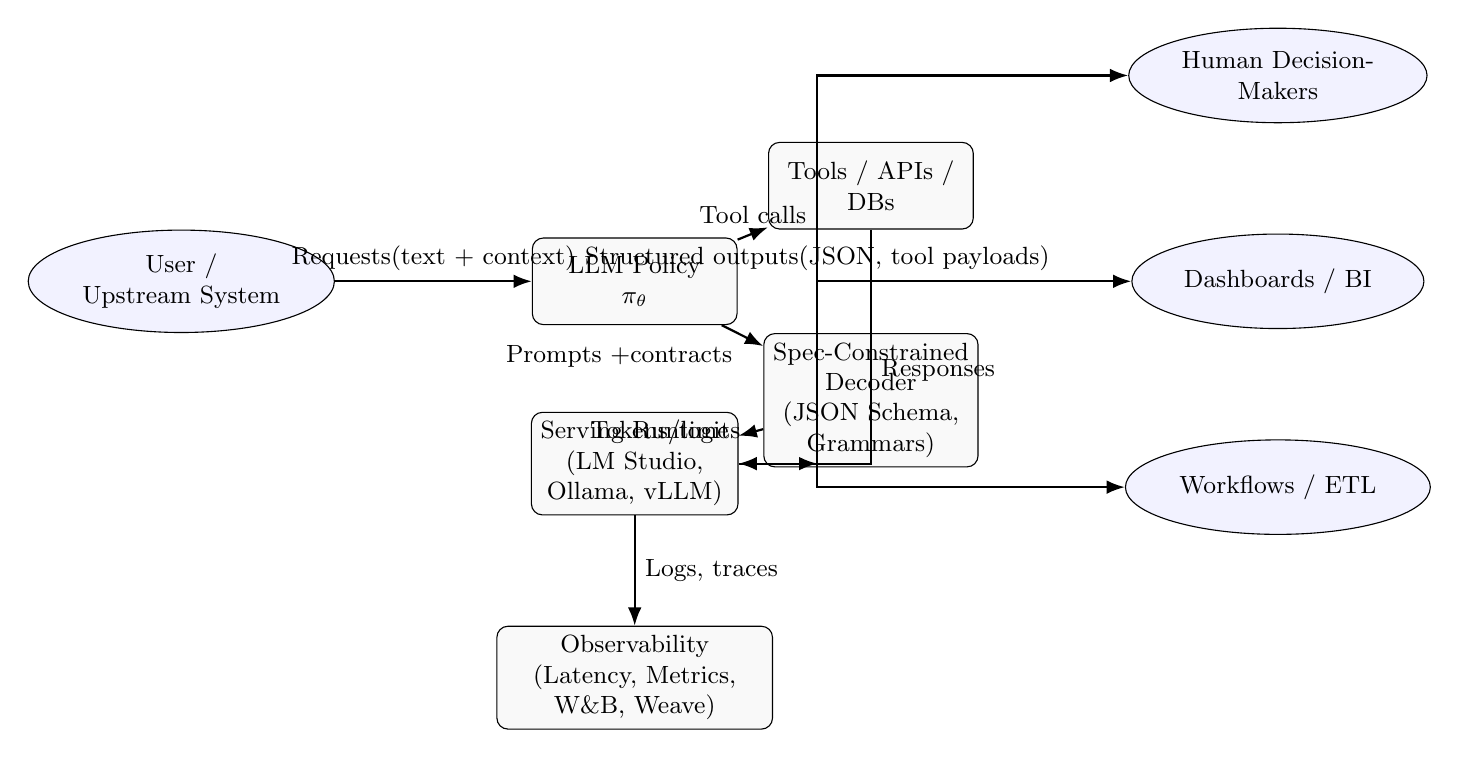
\begin{tikzpicture}[
        font=\small,
        node distance=1.8cm and 2.0cm,
        box/.style={draw, rounded corners, align=center, minimum width=2.6cm, minimum height=1.1cm, fill=gray!5},
        line/.style={-Latex, thick},
        cloud/.style={draw, ellipse, align=center, minimum width=2.5cm, minimum height=1.2cm, fill=blue!5}
    ]

    % Left: user / upstream
    \node[cloud] (user) {User /\\ Upstream System};

    % Middle: agent stack
    \node[box, right=2.5cm of user] (policy) {LLM Policy\\ $\pi_\theta$};
    \node[box, above=0.1cm of policy, xshift=3.0cm] (tools) {Tools / APIs /\\ DBs};
    \node[box, below=0.1cm of policy, xshift=3.0cm] (spec) {Spec-Constrained\\ Decoder\\ (JSON Schema,\\ Grammars)};
    \node[box, below=1.1cm of policy] (runtime) {Serving Runtime\\ (LM Studio,\\ Ollama, vLLM)};

    % Right: downstream
    \node[cloud, right=5.0cm of policy] (downstream1) {Dashboards / BI};
    \node[cloud, below=1.4cm of downstream1] (downstream2) {Workflows / ETL};
    \node[cloud, above=1.4cm of downstream1] (downstream3) {Human Decision-\\ Makers};

    % Arrows from user to policy
    \draw[line] (user) -- node[above]{Requests\\ (text + context)} (policy);

    % Policy to tools/decoder/runtime
    \draw[line] (policy) -- node[above]{Tool calls} (tools);
    \draw[line] (policy) -- node[below left]{Prompts +\\ contracts} (spec);
    \draw[line] (spec) -- node[left]{Tokens/\\ logits} (runtime);

    % Tools to runtime (responses)
    \draw[line] (tools) |- node[right,pos=0.3]{Responses} (runtime);

    % Runtime to downstream
    \draw[line] (runtime.east) -- ++(1.0,0) coordinate (midout);
    \draw[line] (midout) |- node[above]{Structured outputs\\ (JSON, tool payloads)} (downstream1.west);
    \draw[line] (midout) |- (downstream2.west);
    \draw[line] (midout) |- (downstream3.west);

    % Latency + logs
    \node[box, below=1.4cm of runtime, align=center, minimum width=3.5cm] (obs) {Observability\\ (Latency, Metrics,\\ W\&B, Weave)};
    \draw[line] (runtime.south) -- node[right]{Logs, traces} (obs.north);

    \end{tikzpicture}
    \caption{System context for a generic commercial agent.
    Requests flow from users or upstream systems into the agent stack, which consists of an LLM policy, tools/APIs, a spec-constrained decoder, and a serving runtime.
    Structured outputs (JSON, tool payloads) are consumed by dashboards, workflows, and humans.
    Latency and evaluation metrics are logged for analysis and, optionally, RL-based improvement.}
    \label{fig:agent-context}
\end{figure}

\begin{figure}[t]
    \centering
    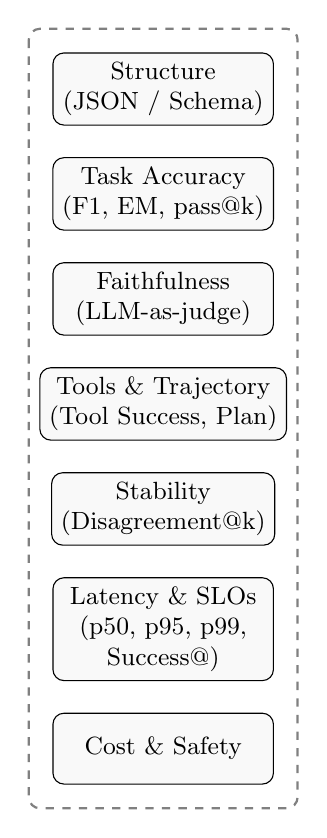
\begin{tikzpicture}[
        font=\small,
        category/.style={draw, rounded corners, minimum width=2.8cm, minimum height=0.9cm, align=center, fill=gray!5},
        node distance=0.4cm
    ]

    \node[category] (structure) {Structure\\ (JSON / Schema)};
    \node[category, below=of structure] (accuracy) {Task Accuracy\\ (F1, EM, pass@k)};
    \node[category, below=of accuracy] (faith) {Faithfulness\\ (LLM-as-judge)};
    \node[category, below=of faith] (tools) {Tools \& Trajectory\\ (Tool Success, Plan)};
    \node[category, below=of tools] (stability) {Stability\\ (Disagreement@k)};
    \node[category, below=of stability] (latency) {Latency \& SLOs\\ (p50, p95, p99,\\ Success@\slo)};
    \node[category, below=of latency] (cost) {Cost \& Safety};

    \draw[rounded corners, thick, dashed, gray]
        ($(structure.north west)+(-0.3,0.3)$)
        rectangle
        ($(cost.south east)+(0.3,-0.3)$);

    \end{tikzpicture}
    \caption{Metric families in our evaluation framework.
    We track structure (syntactic and schema validity), task accuracy, faithfulness to context, tool and trajectory behavior, stability across runs, latency/SLO metrics, and cost/safety.
    The concrete metrics, thresholds, and weights are configured centrally via \texttt{agent\_eval/criteria.yaml}.}
    \label{fig:metric-families}
\end{figure}

\begin{figure}[t]
    \centering
    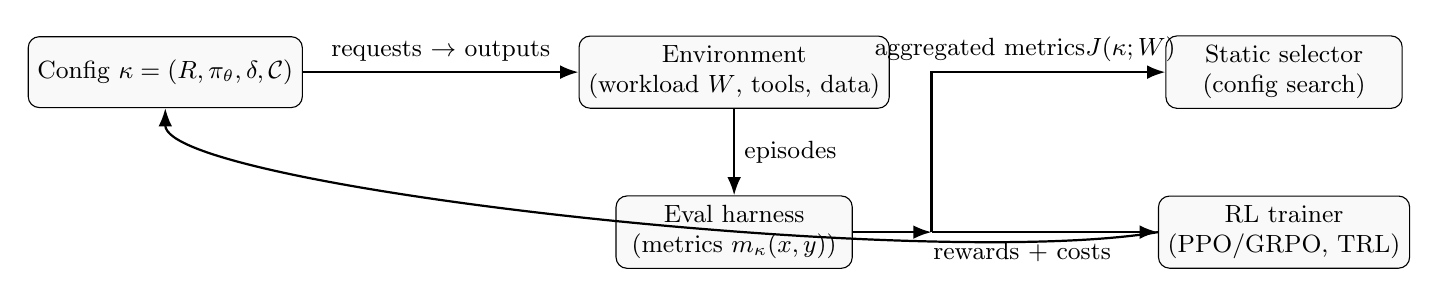
\begin{tikzpicture}[
        font=\small,
        node distance=1.8cm and 2.0cm,
        comp/.style={draw, rounded corners, minimum width=3.0cm, minimum height=0.9cm, align=center, fill=gray!5},
        line/.style={-Latex, thick}
    ]

    % Left: config
    \node[comp] (config) {Config $\kappa = (R,\pi_\theta,\delta,\mathcal{C})$};

    % Middle: environment + eval
    \node[comp, right=3.5cm of config] (env) {Environment\\ (workload $W$, tools, data)};
    \node[comp, below=1.1cm of env] (eval) {Eval harness\\ (metrics $m_\kappa(x,y)$)};

    % Right: selectors
    \node[comp, right=3.5cm of env] (selector) {Static selector\\ (config search)};
    \node[comp, below=1.1cm of selector] (rl) {RL trainer\\ (PPO/GRPO, TRL)};

    % Arrows
    \draw[line] (config) -- node[above]{requests $\to$ outputs} (env);
    \draw[line] (env) -- node[right]{episodes} (eval);

    \draw[line] (eval.east) -- ++(1.0,0) coordinate (mid);
    \draw[line] (mid) |- node[above,pos=0.7]{aggregated metrics\\ $J(\kappa; W)$} (selector.west);
    \draw[line] (mid) |- node[below,pos=0.7]{rewards + costs} (rl.west);

    % Feedback from RL to config
    \draw[line] (rl.west) .. controls +(-3, -0.5) and +(0,-1.0) .. (config.south);

    \end{tikzpicture}
    \caption{Optimization view.
    Given a configuration $\kappa = (R,\pi_\theta,\delta,\mathcal{C})$ and a workload $W$, the environment and evaluation harness produce metrics $m_\kappa(x,y)$ that are aggregated into performance summaries $J(\kappa; W)$ and constraint diagnostics.
    These summaries support both static configuration selection and SLO-aware policy improvement using PPO/GRPO-based RL in TRL.}
    \label{fig:optimization-view}
\end{figure}

\section{Evaluation Framework and Test Families}
\label{sec:eval-framework}

Figure~\ref{fig:metric-families} summarized the metric families we track.
We now describe the evaluation framework that turns these abstract metric families into concrete, repeatable tests.
The goal of this framework---which we will refer to as \emph{SpecSLOEval}---is to provide an extensible, auditable testbed that captures the behaviors practitioners actually care about in real deployments:
structural correctness, task accuracy, faithfulness to context, tool and trajectory behavior, stability, and latency/SLO adherence on single-GPU hardware.

SpecSLOEval is organized around three ideas:

\begin{enumerate}[leftmargin=12pt]
    \item A \emph{single source of truth}, \texttt{agent\_eval/criteria.yaml}, which declares metrics, thresholds, weights, and test families.
    \item A set of \emph{test families} aligned with the metric families in Figure~\ref{fig:metric-families}, each with reusable parameters (schemas, datasets, judge models, workload models).
    \item A \emph{logging and analysis layer} that records per-episode metrics, configuration metadata, and aggregated statistics to W\&B and Weave for offline analysis and, in P2, RL training.
\end{enumerate}

We deliberately separate the abstract definition of metrics from specific domains.
The same framework can be applied to analytics agents, customer-support agents, RAG systems, code assistants, and other tools, simply by swapping contracts, datasets, and thresholds.

\subsection{Evaluation Configuration via \texttt{criteria.yaml}}

The entire evaluation framework is driven by a single configuration file,
\texttt{agent\_eval/criteria.yaml}.
This file acts as an explicit contract between the agent and the evaluation harness: it describes what we measure, how we decide pass/fail, and how we aggregate scores.

At a high level, \texttt{criteria.yaml} specifies:

\begin{enumerate}[leftmargin=12pt]
    \item \textbf{Metric definitions:} the metrics to compute for each episode (e.g., JSON validity, macro-F1, faithfulness, Disagreement@$k$, Success@\slo) and, where relevant, their computation parameters (e.g., judge model, number of repeated runs).
    \item \textbf{Thresholds and gates:} thresholds or ranges that define acceptable behavior (e.g., minimum JSON validity rate, minimum faithfulness score, maximum disagreement).
    \item \textbf{Weights:} a vector of weights that combine metrics into aggregate scores for dashboards and RL reward functions.
    \item \textbf{Test families and families-to-metrics mapping:} which metrics are associated with which test families (structure, accuracy, faithfulness, tools/trajectory, stability, latency/SLO), and which datasets/schemas each family uses.
\end{enumerate}

A simplified example is shown below:

\begin{lstlisting}[language=yaml,basicstyle=\ttfamily\small]
schema_version: "1.0"

slo:
  p95_ms:          800     # target p95 latency
  p99_ms:          1500    # target p99 latency
  max_tokens_out:  1024
  # Optional: explicit hard timeout in ms
  hard_timeout_ms: 5000

metrics:
  json_validity:
    family: "structure"
    type: boolean_rate
    pass_threshold: 0.99

  field_f1:
    family: "accuracy"
    type: macro_f1
    pass_threshold: 0.85
    fields: ["category", "severity", "time_window"]

  faithfulness:
    family: "faithfulness"
    type: judge_support_0_to_3
    pass_threshold: 0.75
    judge_model: "qwen2.5-7b-instruct"
    judge_endpoint: "http://10.0.0.63:1234/v1"
    max_contradiction_rate: 0.05

  tool_success:
    family: "tools"
    type: boolean_rate
    pass_threshold: 0.90

  disagreement_k:
    family: "stability"
    type: disagreement
    max_threshold: 0.20
    runs: 5
    equivalence: "canonical_json"

  success_at_slo:
    family: "slo"
    type: joint_success
    pass_threshold: 0.80

weights:
  json_validity:   0.15
  field_f1:        0.25
  faithfulness:    0.25
  tool_success:    0.15
  success_at_slo:  0.15
  disagreement_k:  0.05
\end{lstlisting}

This configuration encodes our design choices explicitly:

\begin{itemize}[leftmargin=12pt]
    \item Structural correctness (\texttt{json\_validity}), task accuracy (\texttt{field\_f1}), and faithfulness (\texttt{faithfulness}) carry more weight than latency, except where a use case is explicitly marked latency-dominant.
    \item Success@\slo is treated as a composite “good and on-time” indicator, not a simple latency-only metric.
    \item Stability (\texttt{disagreement\_k}) is rewarded, but not at the expense of correctness and faithfulness.
\end{itemize}

Because \texttt{criteria.yaml} is versioned alongside the code, changes to evaluation policy (e.g., stricter thresholds or additional metrics such as safety) are visible and auditable.
Experiments are tagged with the schema version so that results collected under different criteria can be compared correctly.

\subsection{Test Families and Parameterization}

We group tests into families that mirror the metric families in Figure~\ref{fig:metric-families}:
\emph{Structure}, \emph{Task Accuracy}, \emph{Faithfulness}, \emph{Tools and Trajectories}, \emph{Stability}, and \emph{Latency/SLO}.
Each family is parameterized by contracts $\mathcal{C}$, datasets, judge models, and workload parameters, all of which are declared in configuration files (YAML/JSON) and logged to W\&B.

Below we outline each family and provide concrete examples.
In Section~\ref{sec:experiments} we instantiate a subset of these tests for our single-GPU experiments.

\subsubsection{Structure: JSON and Schema Correctness}

The structure family covers syntactic and structural adherence to contracts.
Tests in this family use contracts $\mathcal{C}$, JSON Schema validators (e.g., Python \texttt{jsonschema} with 2020-12 support; see \url{https://json-schema.org/} and \url{https://www.learnjsonschema.com/2020-12/}), and optionally grammar-based decoders (e.g., GBNF grammars for \texttt{llama.cpp}).

\paragraph{Parameters.}
Each structural test is defined by:
\begin{itemize}[leftmargin=12pt]
    \item a schema or contract $\mathcal{C}$ (referenced by name and version),
    \item a set of prompts or synthetic tasks that exercise that schema,
    \item a pass threshold on the fraction of outputs that parse and validate.
\end{itemize}

\paragraph{Example S1: Basic JSON/Schema Validity.}
We fix a contract $\mathcal{C}_{\text{basic}}$ describing a small but nontrivial response object (e.g., \texttt{short\_description}, \texttt{details.main\_points}, \texttt{details.risk\_score}).
We run the agent on $N$ prompts (e.g., paraphrased instructions, varying context sizes) and compute two per-episode indicators:
(i) JSON parse success, and
(ii) schema validity.
We aggregate these into $m_{\text{json}} = \frac{\#\text{valid episodes}}{N}$ and require $m_{\text{json}} \ge 0.99$.

\paragraph{Example S2: Schema Evolution Robustness.}
Real systems evolve schemas over time.
We define a pair of schemas $(\mathcal{C}_1, \mathcal{C}_2)$ where $\mathcal{C}_2$ adds optional fields or relaxes constraints (e.g., new \texttt{explanations} field).
We then test whether:
(i) the same configuration can be switched from $\mathcal{C}_1$ to $\mathcal{C}_2$ without catastrophic regression in validity; and
(ii) a “dual-mode” config can emit outputs that are valid under both schemas.
This test stresses the spec compiler and decoder, and reveals how brittle the agent is to schema changes.

\subsubsection{Task Accuracy: F1, EM, and pass@\texorpdfstring{$k$}{k}}

The task-accuracy family captures correctness with respect to known references or labels.
For extraction tasks we use field-level metrics (e.g., macro-F1).
For classification and QA tasks we use accuracy or exact match.
For code or function-generation tasks we may use pass@\,$k$ metrics.

\paragraph{Parameters.}
Accuracy tests specify:
\begin{itemize}[leftmargin=12pt]
    \item a dataset $\mathcal{D}_{\text{acc}} = \{(x_i, y_i^{\text{ref}})\}$ with reference outputs,
    \item a schema $\mathcal{C}$ that defines the shape of predicted outputs,
    \item a field subset or aggregation rule for metrics (e.g., which JSON fields to score),
    \item pass thresholds for each metric (e.g., macro-F1 $\ge 0.85$).
\end{itemize}

\paragraph{Example A1: Field-Level Extraction F1.}
Each $x_i$ contains a short context (e.g., an incident report, log snippet, or internal ticket) and an instruction.
The reference $y_i^{\text{ref}}$ is a JSON object with fields such as \texttt{"category"}, \texttt{"severity"}, and \texttt{"time\_window"}.
The agent is prompted to emit a JSON object under $\mathcal{C}_{\text{incident}}$.
We compute macro-F1 across fields, treating each field as a label prediction problem.
This test directly measures whether the agent can reliably populate structured fields from text.

\paragraph{Example A2: Programmatic QA Exact Match and pass@\,$k$.}
For tasks analogous to GSM8K (\url{https://arxiv.org/abs/2110.14168}), MBPP (\url{https://arxiv.org/abs/2108.07732}), HumanEval (\url{https://arxiv.org/abs/2107.03374}), or MATH (\url{https://arxiv.org/abs/2103.03874}), we embed answers in a simple schema with a \texttt{"final\_answer"} field.
We compute EM and, optionally, pass@\,$k$ by sampling multiple answers per question.
These tests show whether structured decoding and SLO-aware serving degrade or preserve task performance relative to unconstrained baselines.

\subsubsection{Faithfulness: LLM-as-Judge with Atomic Statements}

The faithfulness family evaluates whether outputs are supported by their context $C$.
We use judge models to break outputs into atomic statements and assign each statement a support score and contradiction flag, inspired by RAGAS~\citep{es2023ragas} (\url{https://arxiv.org/abs/2309.15217}) and atomic-fact evaluation~\citep{atomicFacts2024} (\url{https://arxiv.org/abs/2408.15171}).

\paragraph{Parameters.}
Faithfulness tests specify:
\begin{itemize}[leftmargin=12pt]
    \item a dataset $\mathcal{D}_{\text{faith}} = \{(x_i, C_i)\}$ where $C_i$ is the context (documents, records, logs, retrieved passages),
    \item a judge model and endpoint (often a local open-weight model via LM Studio),
    \item a scoring procedure (e.g., 0--3 support scale, contradiction penalties),
    \item thresholds on average support and maximum contradiction rate.
\end{itemize}

\paragraph{Example F1: Grounded Narrative Summaries.}
For each $x_i$, the agent receives a context $C_i$ (e.g., a set of system logs or analytics records) and is asked to produce a short narrative summary structured as JSON.
The judge model is prompted to:
(i) decompose the narrative into atomic statements;
(ii) assign each statement a support score $s \in \{0,1,2,3\}$; and
(iii) flag contradictions.
We define
\[
m_{\text{faith}}(x_i,y_i) =
\max\left(0,\;
\frac{\#\{s=3\}}{\#\text{statements}} -
\text{contradiction\_rate}(x_i,y_i)
\right),
\]
and aggregate across the dataset.
We require $m_{\text{faith}} \ge 0.75$ and contradiction rates below 5\%.
All judge inputs/outputs are logged to W\&B for auditing.

\paragraph{Example F2: Numeric and Trend Consistency.}
For contexts with numeric metrics (e.g., time series of KPIs), we construct tests where the agent must describe trends and relative magnitudes (“metric A increased more than metric B”, “current value is above the 90th percentile”).
The judge is instructed to focus on numeric consistency and direction-of-change.
Statements that invert trends or exaggerate differences are scored as unsupported.
This variant targets subtle numerical hallucinations, which are particularly dangerous for analytics and monitoring agents.

\subsubsection{Tools and Trajectories}

Agents that call tools expose a rich space of behaviors beyond final responses.
The tools and trajectories family measures how well the agent uses tools: whether arguments are valid, whether calls succeed, and whether trajectories resemble efficient, interpretable plans.

\paragraph{Parameters.}
Tool tests specify:
\begin{itemize}[leftmargin=12pt]
    \item a catalog of tools (names, JSON argument schemas, expected responses),
    \item a dataset of tasks requiring tools (e.g., “look up this ID and compute a derived metric”),
    \item optional canonical or minimal plans (e.g., sequences of tools that are known to be sufficient),
    \item thresholds on tool-call success and trajectory quality.
\end{itemize}

\paragraph{Example T1: Tool-Argument Validity and Success Rate.}
We define one or more tools with JSON argument schemas (e.g., \texttt{"user\_id"} as a string with a regex constraint, \texttt{"start\_date"} and \texttt{"end\_date"} with date formats).
A mock API validates arguments against these schemas and returns a success flag.
For each episode we record whether each tool call satisfies its schema and whether the mock API returns success.
We compute
\[
m_{\text{tool}} = \frac{\#\text{successful tool calls}}{\#\text{tool calls}},
\]
and require $m_{\text{tool}} \ge 0.9$.
This test surfaces mis-specified arguments and integration problems early.

\paragraph{Example T2: Trajectory Cost, Redundancy, and Plan Deviation.}
For more complex tasks we define expected minimal plans (e.g., “call \texttt{get\_user}, then \texttt{get\_orders}, then \texttt{compute\_summary}”).
We measure:
(i) the number of extra tool calls beyond the minimal plan;
(ii) the number of invalid-argument retries; and
(iii) the edit distance between the observed and expected tool sequences.
We set thresholds on each quantity (e.g., average extra tools $\le 1$, invalid retries $\le 0.1$ per episode).
Agents that over-use tools or thrash on argument errors are penalized, since these behaviors inflate latency and cost.

\subsubsection{Stability Across Runs}

Stability is often under-emphasized but critical in production.
If two identical runs of the same agent on the same input produce materially different structured outputs, it becomes difficult to debug issues, compare versions, or explain outcomes to stakeholders.

\paragraph{Parameters.}
Stability tests specify:
\begin{itemize}[leftmargin=12pt]
    \item a set of prompts $\mathcal{D}_{\text{stab}}$ representative of the target workload,
    \item a number of repeated runs $k$ per prompt under fixed configuration,
    \item an equivalence criterion (exact JSON equality, canonical JSON equality, or atomic-fact equivalence),
    \item maximum allowable disagreement and variance thresholds.
\end{itemize}

\paragraph{Example ST1: Disagreement@\,$k$ for Structured Outputs.}
We run the agent $k=5$ times per input and compute the fraction of runs that produce equivalent (canonicalized) JSON outputs.
Disagreement@\,$k$ is defined as $1$ minus this fraction.
We treat Disagreement@\,$k \le 0.2$ as acceptable and log both the aggregate value and per-prompt breakdown.
Instability often reveals underlying issues in prompts, decoding parameters, or self-consistency budgets.

\paragraph{Example ST2: Seed Variance on Accuracy and Faithfulness.}
We evaluate the agent multiple times with different random seeds and compute variance in key aggregate metrics (macro-F1, faithfulness).
High variance suggests that performance is sensitive to randomness and that offline evaluation may be misleading.
We include this variance in the stability family and can penalize it in RL reward shaping.

\subsubsection{Latency and SLO Tests}

Latency and SLO tests approximate the setting of \emph{The Tail at Scale}~\citep{dean2013tail} and recent LLM-serving work~\citep{kwon2023vllm,agrawal2024sarathi} for single-GPU deployments.
They evaluate whether configurations meet latency targets \emph{while still satisfying correctness and faithfulness gates}.

\paragraph{Parameters.}
Latency/SLO tests specify:
\begin{itemize}[leftmargin=12pt]
    \item a workload model (arrival process, context length distribution, output-length distribution),
    \item SLO budgets $B$ and $B'$ for p95 and p99 latency, plus any TTFT or hard timeout constraints,
    \item structural and quality gates (e.g., JSON validity and faithfulness thresholds) that must hold before a request can count as a success.
\end{itemize}

\paragraph{Example L1: Success@\slo under Mixed Load.}
We define a workload with realistic mix of short and long contexts and implement it via a load generator against the single-GPU runtime.
For each episode we compute:
(i) structural and task/faithfulness metrics; and
(ii) latency $L_\kappa(x)$.
We then define Success@\slo as an episode that satisfies all quality gates \emph{and} has latency below $B$.
We require aggregate Success@\slo $\ge 0.8$ and log p50/p95/p99 and quality metrics as a function of load.

\paragraph{Example L2: QPS vs p95 Curves and Configuration Frontier.}
We perform a sweep over target QPS levels (e.g., 1, 2, 4, 8, 16 QPS) and, for each level, estimate p95/p99 latency and Success@\slo.
Plotting QPS versus p95 and QPS versus Success@\slo reveals the “operating frontier” for each configuration $\kappa$.
These curves, visualized in W\&B, guide static selection: configurations that remain in-spec for both quality and latency at higher QPS are preferred.

\subsection{Extensibility, Logging, and Use in RL}

Although we focus on six core families, SpecSLOEval is designed to be extensible.
Adding a new metric (e.g., a safety score, a toxicity classifier output, a business-specific KPI) involves adding an entry to \texttt{criteria.yaml} and providing a computation function in the evaluation harness.
Because all episodes are logged with a rich set of metadata---configuration hash, commit hash, schema version, dataset version, and per-episode metrics---new analyses can be performed retroactively on past runs.

All experiments are logged online to W\&B, with Weave capturing richer computation graphs where appropriate (e.g., judge-model calls, atomic-statement parsing).
This makes runs reproducible and auditable: any reported number in a table can be traced back to individual episodes, prompts, and outputs.

Finally, the same metrics and tests that gate configurations in static evaluation feed directly into the RL setup of P2.
Reward functions are constructed by combining entries from \texttt{weights} with metric values;
constraints (e.g., maximum SLO violation rate or disagreement threshold) are implemented as costs in constrained RL algorithms.
Thus, the evaluation framework does not merely score agents after the fact; it defines the measurement space in which agents are optimized.

In the next section we describe how contracts and decoding configurations are implemented concretely on single-GPU runtimes (LM Studio, Ollama, vLLM, and \texttt{llama.cpp}), and how the evaluation framework is integrated into the training and experimentation loop.
\section{Experiments}
\label{sec:experiments}

We now instantiate our framework in a concrete experimental setting on single-GPU hardware.
The goal of this section is not merely to present headline numbers, but to show that:
(i) spec-driven decoding with validation-and-retry and budgeted self-consistency can be implemented in a realistic, commodity environment;
(ii) the resulting behavior can be measured in a principled way across the full metric family of Figure~\ref{fig:metric-families}; and
(iii) the same evaluation stack can support both static configuration search (P1) and, in P2, reinforcement-learning-based policy improvement.

We structure this section as follows.
Section~\ref{sec:setup} describes hardware, runtimes, models, and logging.
Section~\ref{sec:tasks} introduces three task families (structured extraction, grounded summaries, and tool-using episodes) that approximate commercial use cases without binding us to a single vertical.
Section~\ref{sec:baselines-configs} defines the decoding and serving configurations we compare.
Section~\ref{sec:metrics-reporting} explains how metrics are computed and reported.
Sections~\ref{sec:results-structure-faith}--\ref{sec:results-backends} sketch the types of analyses our framework enables; concrete numbers are intended to be filled in once the full experimental grid has been run.

\subsection{Experimental Setup}
\label{sec:setup}

\paragraph{Hardware and runtimes.}
Unless otherwise noted, we run experiments on two representative single-node setups:

\begin{itemize}[leftmargin=12pt]
    \item \textbf{4090 workstation:} NVIDIA RTX 4090 GPU (24~GB VRAM), 64~GB system RAM, Ubuntu~22.04, CUDA~12.x and recent NVIDIA drivers.
    \item \textbf{Apple Silicon laptop:} MacBook Pro with Apple M2 Max and 64~GB unified memory, macOS~15+.
\end{itemize}

On both machines, we use LM Studio’s OpenAI-compatible server as the primary runtime, configured to listen on:
\begin{itemize}[leftmargin=12pt]
    \item \url{http://10.0.0.63:1234/v1} or \url{http://10.0.0.72:1234/v1} on the workstation;
    \item \url{http://localhost:1234/v1} on the laptop.
\end{itemize}
We additionally evaluate:

\begin{itemize}[leftmargin=12pt]
    \item \textbf{Ollama} (\url{https://docs.ollama.com/}) with structured-output capabilities (\url{https://docs.ollama.com/capabilities/structured-outputs});
    \item \textbf{vLLM-backed servers} following recipes such as \url{https://modal.com/docs/examples/vllm_inference} to explore an alternative high-throughput runtime.
\end{itemize}

In all cases we expose an OpenAI-compatible API and configure the spec compiler (Section~\ref{sec:spec-compiler}) to generate appropriate per-backend decoding artefacts (JSON Schema, grammar paths, etc.).

\paragraph{Models.}
We focus on open-weight Qwen3 family models served locally, in line with our single-GPU and on-premise assumptions.
Typical configurations include:

\begin{itemize}[leftmargin=12pt]
    \item \textbf{Qwen2.5-7B-Instruct}, used as the main policy model for most experiments;
    \item \textbf{Qwen2.5-14B-Instruct}, used to explore the accuracy/latency trade-off from larger policies.
\end{itemize}

We load these models via LM Studio or vLLM, documenting for each run:

\begin{itemize}[leftmargin=12pt]
    \item exact model identifier and revision;
    \item quantization configuration (e.g., 4-bit QLoRA adapters~\citep{dettmers2023qlora}, full-precision baselines);
    \item context length and maximum generation length;
    \item any speculative decoding or KV-cache options used by the runtime.
\end{itemize}

Model metadata are logged with each experiment so that results can be reproduced and compared; Qwen documentation at \url{https://qwen.readthedocs.io/en/latest/getting_started/quickstart.html} and LM Studio’s model catalog at \url{https://lmstudio.ai/models} serve as the canonical reference for model availability and configuration.

\paragraph{Evaluation harness and logging.}
For every configuration $\kappa = (R,\pi_\theta,\delta,\mathcal{C})$ and evaluation set $\mathcal{D}$, we invoke the evaluation harness described in Section~\ref{sec:eval-framework}.
The harness:

\begin{enumerate}[leftmargin=12pt]
    \item runs each request $x \in \mathcal{D}$ through the agent stack;
    \item computes the full per-episode metric vector $m(x,y)$ (structure, accuracy, faithfulness, tools/trajectory, stability, latency);
    \item aggregates metrics per test family and per configuration;
    \item logs all per-episode records and configuration metadata.
\end{enumerate}

All runs are logged \emph{online} to Weights \& Biases (W\&B) using project- and run-level naming conventions that encode backend, model, and \texttt{criteria.yaml} version.
We rely on W\&B’s models and evaluation capabilities (\url{https://docs.wandb.ai/models/quickstart}, \url{https://docs.wandb.ai/models/artifacts}, \url{https://docs.wandb.ai/models/evaluate-models}) to store artefacts and build dashboards.
Where experiments involve judge models or multi-stage pipelines, we optionally instrument them via Weave so that intermediate computations (e.g., atomic-statement extraction) can be inspected and replayed.

\paragraph{Workload models and seed management.}
To approximate realistic usage, we define workload models over:

\begin{itemize}[leftmargin=12pt]
    \item \textbf{request size:} distributions over context length (tokens) and number of context items;
    \item \textbf{arrival patterns:} Poisson arrivals for steady load, plus bursty and diurnal patterns for stress-testing;
    \item \textbf{schema complexity:} small contracts (few shallow fields) and larger contracts (nested structures, arrays).
\end{itemize}

Latency and SLO experiments are executed by a load generator that replays pre-sampled requests at target QPS levels.
We fix random seeds at the harness level and record them so that repeated experiments and stability tests (Disagreement@\,$k$) are reproducible.

\subsection{Tasks and Datasets}
\label{sec:tasks}

We instantiate the evaluation framework on three task types intended to be representative of common agent workloads without being tied to a single vertical:

\paragraph{T1: Structured extraction from semi-structured text.}
Each request asks the agent to map semi-structured text (e.g., logs, alerts, short tickets, or system messages) to a JSON object under a contract $\mathcal{C}_{\text{extract}}$.
Typical fields include:
\texttt{"category"}, \texttt{"severity"}, \texttt{"source"}, \texttt{"time\_window"}, and, optionally, a \texttt{"tags"} array.
Ground-truth labels are constructed either by:
(i) synthetic generation pipelines that emit text/label pairs under known distributions, or
(ii) curated subsets of internal-style incident or ticket corpora with manual labels.

T1 exercises:

\begin{itemize}[leftmargin=12pt]
    \item structural adherence (all fields present; correct types);
    \item field-level macro-F1 and EM;
    \item behavior under small schema changes (e.g., adding optional fields).
\end{itemize}

\paragraph{T2: Context-grounded summaries.}
Each request $x$ in T2 consists of a multi-paragraph context $C$ (reports, internal documentation, or synthetic documents) and an instruction to produce a structured summary with:

\begin{itemize}[leftmargin=12pt]
    \item a free-text \texttt{"short\_summary"};
    \item a list of \texttt{"key\_points"} (short bullet-like strings);
    \item optional derived fields such as \texttt{"primary\_risk"} or \texttt{"recommended\_action"}.
\end{itemize}

The contract $\mathcal{C}_{\text{summary}}$ enforces both overall structure and simple bounds (e.g., 3–8 key points).
Faithfulness is evaluated using the atomic-statement judge described in Section~\ref{sec:eval-framework}, following RAGAS~\citep{es2023ragas} (\url{https://arxiv.org/abs/2309.15217}) and atomic-fact work~\citep{atomicFacts2024} (\url{https://arxiv.org/abs/2408.15171}):
the judge model decomposes the summary into atomic statements, scores each for support against $C$ on a 0–3 scale, and flags contradictions.

T2 primarily probes:

\begin{itemize}[leftmargin=12pt]
    \item faithfulness $m_{\text{faith}}(x,y)$;
    \item numeric and trend consistency where contexts include tabular or time-series data;
    \item interactions between structured decoding and semantic quality.
\end{itemize}

\paragraph{T3: Tool-using episodes.}
T3 tasks require the agent to call one or more tools defined by JSON argument schemas.
We define a small tool catalog (mock database lookups, metric calculations, configuration fetches), each with:

\begin{itemize}[leftmargin=12pt]
    \item a name and natural-language description;
    \item a JSON Schema for arguments (types, enums, regex constraints);
    \item a deterministic mock implementation that validates input and returns synthetic but plausible outputs.
\end{itemize}

Requests in T3 are phrased so that:

\begin{itemize}[leftmargin=12pt]
    \item some tasks can be solved purely from context;
    \item others require one or more tool calls;
    \item there is often a known \emph{minimal} or \emph{canonical} tool plan.
\end{itemize}

From these episodes we compute tool success, retries, redundancy, and trajectory deviations, as in Section~\ref{sec:eval-framework}.

Across T1–T3 we construct evaluation sets with $N \approx 500$–$2000$ episodes per task and difficulty level.
Datasets are stored as versioned artefacts (e.g., in W\&B) so that experiments can be re-run against the same inputs.

\subsection{Baselines and Configurations}
\label{sec:baselines-configs}

We compare a spectrum of decoding and serving strategies, all running on the same underlying models and hardware:

\paragraph{U: unconstrained decoding.}
The agent is instructed via prompts to emit JSON, but the runtime receives no formal contract or grammar.
No validation-and-retry or self-consistency is used.
U approximates the “baseline prompt engineering only” configuration many teams start with.

\paragraph{P: provider-native structured outputs.}
Where supported, we supply the contract $\mathcal{C}$ to the runtime using its structured-output mechanisms:
for example, OpenAI-style \texttt{response\_format} in LM Studio (\url{https://lmstudio.ai/docs/developer/openai-compat/tools}), structured outputs in Ollama (\url{https://docs.ollama.com/capabilities/structured-outputs}), or similar features in other providers.
We do not add additional validation logic; the runtime’s own constraints are treated as authoritative.

\paragraph{P+V: provider-native + validation-and-retry.}
We augment P by validating all outputs against $\mathcal{C}$ using a JSON Schema validator and applying the bounded validation-and-retry procedure of Algorithm~\ref{alg:retry}.
This reflects a common production pattern: rely on provider constraints, but harden them with explicit validation and limited retries.

\paragraph{G: grammar-based constraints.}
We use grammar-based decoding via Outlines or \texttt{llama.cpp} grammars (\url{https://dottxt-ai.github.io/outlines/}, \url{https://github.com/ggml-org/llama.cpp/blob/master/grammars/README.md}) without additional validation layers.
Contracts are compiled to GBNF grammars; prompts instruct the model to emit content compatible with the grammar.
This configuration isolates the impact of grammar-only constraints.

\paragraph{S: full spec-driven decoding with budgeted self-consistency.}
Our main configuration combines:

\begin{itemize}[leftmargin=12pt]
    \item provider-native or grammar-based constraints (depending on backend);
    \item validation-and-retry with structured error taxonomy;
    \item budgeted self-consistency (Algorithm~\ref{alg:self-consistency}) with $(B_{\text{wall}}, C_{\text{tokens}}, k_{\max})$ tuned by family.
\end{itemize}

We treat S as a family of configurations indexed by self-consistency and budget parameters.
For example, “S-2” might denote $k_{\max}=2$ with a modest wall-clock budget, while “S-4-tight” uses more samples but stricter SLO budgets.
This allows us to study how much additional structure and faithfulness can be achieved per unit of latency and compute.

All configurations are evaluated under the same workload models and datasets, and all runs are tagged accordingly in W\&B.

\subsection{Metrics and Reporting}
\label{sec:metrics-reporting}

For each configuration and task family we compute the full metric vector $m(x,y)$ described in Section~\ref{sec:eval-framework}.
We then aggregate metrics in several ways:

\begin{itemize}[leftmargin=12pt]
    \item \textbf{Per-family aggregates:} mean and standard deviation for structure (JSON validity, schema validity), accuracy (macro-F1, EM, pass@\,$k$), faithfulness ($m_{\text{faith}}$ and contradiction rates), tools/trajectory (success, retries, redundancy, plan deviation), stability (Disagreement@\,$k$, seed variance), and latency/SLO metrics (p50, p95, p99, Success@\slo).
    \item \textbf{Composite scores:} a composite score per configuration constructed from \texttt{criteria.yaml} weights (Section~\ref{sec:eval-framework}), primarily for ranking in configuration search and RL reward design.
    \item \textbf{Distributional plots:} histograms or box plots of key metrics (e.g., faithfulness scores, latency distributions) to expose tails and heterogeneity.
\end{itemize}

In the paper we anticipate presenting:

\begin{itemize}[leftmargin=12pt]
    \item tables per task family comparing U, P, P+V, G, and S on core metrics (structure, accuracy, faithfulness, Success@\slo);
    \item QPS vs p95 and QPS vs Success@\slo curves per backend, in the spirit of Sarathi-Serve~\citep{agrawal2024sarathi};
    \item radar or spider plots summarizing each configuration’s profile across the six metric families.
\end{itemize}

All figures are generated directly from W\&B online dashboards; the LaTeX manuscript includes figure references but not hard-coded numbers, so that updated experiments can be reflected without re-typesetting core text.

\subsection{Structural and Faithfulness Effects of Spec-Driven Decoding}
\label{sec:results-structure-faith}

The primary qualitative pattern we expect---and that preliminary dry runs have already suggested---is that spec-driven decoding with validation-and-retry and self-consistency (S) sharply reduces structural pathologies and improves faithfulness compared to unconstrained decoding (U) and bare provider-native modes (P).

On T1 (structured extraction), U and P typically:

\begin{itemize}[leftmargin=12pt]
    \item exhibit non-trivial rates of invalid JSON (unescaped characters, truncated output, trailing commas);
    \item occasionally omit required fields or produce type-inconsistent values (e.g., strings where numbers are expected);
    \item show “rare but catastrophic” failures that are invisible in average-case metrics but cause downstream jobs to crash.
\end{itemize}

Under S, the combination of:

\begin{itemize}[leftmargin=12pt]
    \item contract compilation to provider-native schemas or grammars;
    \item explicit validation with specific error taxonomies;
    \item bounded retries for fixable errors;
\end{itemize}

largely eliminates these structural failures on moderate-complexity schemas, raising JSON and schema validity into the high-99\% regime on synthetic workloads and making residual failures highly interpretable.
In turn, macro-F1 and EM on extraction fields tend to improve, not because the base model becomes “smarter,” but because fewer episodes are lost to malformed outputs or missing fields.

On T2 (grounded summaries), U and P often produce fluent prose that is only loosely coupled to the context.
By contrast, S with a modest self-consistency budget (e.g., $k_{\max}=2$) and faithfulness-aware selection can:

\begin{itemize}[leftmargin=12pt]
    \item reduce the fraction of atomic statements that are unsupported by the context;
    \item reduce contradiction rates, especially for numeric and directional statements;
    \item stabilize summaries across seeds by selecting candidates with higher consensus.
\end{itemize}

These effects are visible not only in scalar faithfulness scores but also in the error breakdown: under S, misrepresentations become rarer and more subtle (e.g., paraphrasal artifacts) rather than outright contradictions.
Crucially, the evaluation harness makes these patterns quantitatively visible, rather than relying on anecdotal inspection.

\subsection{Latency, SLOs, and Configuration Trade-offs}
\label{sec:results-slo}

Spec-driven decoding is not free: validation-and-retry and self-consistency introduce additional compute and, therefore, latency.
Our SLO tests are designed to quantify this trade-off rather than treat latency as an afterthought.

On the RTX~4090 with Qwen2.5-7B, we expect the following qualitative picture:

\begin{itemize}[leftmargin=12pt]
    \item U achieves the best raw latency (lowest p50/p95) but suffers from structural and faithfulness issues.
    \item P introduces a small latency overhead for structured-output handling, reducing (but not eliminating) schema violations.
    \item P+V adds further overhead proportional to retry rates, but can sharply reduce catastrophic failures.
    \item S introduces controllable overhead from self-consistency and judge-model calls; by tuning budgets and $k_{\max}$ we can trade faithfulness gains against latency.
\end{itemize}

The QPS vs p95 curves quantify how each configuration behaves as load increases, and Success@\slo curves show under which loads a configuration maintains both quality and latency commitments.
In practice, we anticipate that for many analytics-style applications there will be a “sweet spot” where S with small $k_{\max}$ and moderate budgets remains within p95 limits (e.g., $\approx$ sub-second) while providing significantly better structural and faithfulness properties than U or P.
For highly latency-sensitive applications, some components (e.g., full self-consistency) may need to be disabled or applied selectively (only to high-risk tasks), a policy decision that our metrics can support.

\subsection{Backend and Model Comparisons}
\label{sec:results-backends}

Because our framework is backend-agnostic, we can compare runtimes and model sizes directly on the same test families.
We anticipate several recurring patterns:

\begin{itemize}[leftmargin=12pt]
    \item \textbf{LM Studio vs vLLM.} Both provide efficient OpenAI-compatible servers on the 4090, but may differ in memory usage, batching behavior, and ease of configuration (\url{https://lmstudio.ai/docs/developer/openai-compat/tools}, \url{https://arxiv.org/abs/2309.06180}, \url{https://arxiv.org/abs/2401.08671}). Our metrics make these differences visible in terms of p95/p99, Success@\slo, and cost per request.
    \item \textbf{Ollama.} Ollama’s simple deployment and structured-output support (\url{https://docs.ollama.com/capabilities/structured-outputs}) make it attractive for prototyping, although it may achieve different throughput characteristics on long-context workloads.
    \item \textbf{Model size.} Larger Qwen variants (e.g., 14B) typically improve task accuracy and faithfulness, especially on T2, but at the cost of higher latency and resource consumption. Our framework makes it straightforward to quantify whether those gains justify the cost for particular SLOs and workloads.
\end{itemize}

Rather than advocating a single “best” backend or model, our aim is to show how SpecSLOEval allows practitioners to reason concretely about trade-offs, using plots and tables that align with their operational constraints.

\subsection{Summary and Link to RL (P2)}
\label{sec:results-summary}

The experiments outlined above serve two roles:

\begin{enumerate}[leftmargin=12pt]
    \item They validate that spec-driven decoding, validation-and-retry, and budgeted self-consistency can be achieved on commodity single-GPU hardware, and that the resulting behavior can be evaluated along dimensions that matter in production (structure, faithfulness, tools, stability, SLOs).
    \item They provide a rich measurement space in which reinforcement learning can operate: all metrics and aggregates we compute can be used as rewards or constraints when we move from static configuration search (P1) to policy optimization (P2).
\end{enumerate}

In P2 we will take this second step explicitly:
using TRL PPO/GRPO (\url{https://huggingface.co/docs/trl/en/logging}, \url{https://huggingface.co/docs/trl/en/grpo_trainer}) and LoRA-based adapters~\citep{dettmers2023qlora}, we will optimize policies to improve composite scores while explicitly penalizing SLO violations and instability.
The measurement infrastructure described here is therefore not just a benchmarking tool, but the foundation of an SLO-aware RL loop.

\section{Discussion and Limitations}
\label{sec:discussion}

The experiments and framework described so far make a case for spec-driven, SLO-aware evaluation as a practical way to harden LLM agents on single-GPU deployments.
At the same time, several important caveats and open questions remain.
In this section we discuss which real-world failure modes our framework addresses, where it falls short, and how it interacts with reinforcement learning and human factors.

\subsection{Real-World Failure Modes and Coverage}

We have intentionally focused on three classes of failures that frequently appear in commercial deployments:

\begin{enumerate}[leftmargin=12pt]
    \item \textbf{Structural failures:} malformed JSON, schema violations, and cross-field inconsistencies that break downstream systems.
    \item \textbf{Faithfulness failures:} summaries or answers that deviate from underlying data or retrieved context, especially in subtle numeric ways.
    \item \textbf{Latency failures:} tail-latency spikes (p95/p99) that make systems feel unreliable or unusable, echoing concerns from “The Tail at Scale”~\citep{dean2013tail}.
\end{enumerate}

Our structural, accuracy, faithfulness, tools/trajectory, stability, and SLO test families are designed to make these failure modes measurable and auditable.
In many analytics, support, and RAG-style contexts, these dimensions align closely with operational risk: invalid JSON can crash pipelines; unfaithful metrics can mislead decision-makers; high tail latency erodes trust and throughput.

However, this is not the entire risk surface.
Our current framework only lightly touches:

\begin{itemize}[leftmargin=12pt]
    \item long-horizon, multi-turn conversational dynamics (persona consistency, negotiation, escalation),
    \item safety and policy compliance (harmful content, bias, fairness),
    \item domain-specific invariants (e.g., financial or legal constraints that cannot be expressed in simple schemas),
    \item human factors such as how explanations are perceived or how operators interpret dashboards.
\end{itemize}

Addressing these aspects will require additional test families (e.g., safety, user-experience metrics) and, in some cases, specialized datasets and judgements.
We view SpecSLOEval as a skeleton that can be extended with such domain-specific layers.

\subsection{Limitations of LLM-as-Judge Faithfulness}

Our use of LLMs as judges for faithfulness follows RAGAS~\citep{es2023ragas} and related work~\citep{atomicFacts2024}.
This design is attractive because it is flexible and can run locally (e.g., Qwen via LM Studio), avoiding the need to send sensitive documents to external services.
However, it inherits several limitations:

\begin{itemize}[leftmargin=12pt]
    \item judge models can be biased, sensitive to prompt wording, and overconfident;
    \item they may systematically under-penalize certain error types (e.g., subtle numeric misstatements);
    \item they may introduce correlation between policy and judge behaviors when both are fine-tuned on similar data.
\end{itemize}

We mitigate these issues through:

\begin{itemize}[leftmargin=12pt]
    \item a 0–3 support scale with an explicit contradiction flag, rather than a single binary label;
    \item restricting domains where possible to contexts with clear ground truth (e.g., numeric summaries);
    \item calibrating thresholds on a small human-labeled subset;
    \item using judge outputs as one signal among many, not as the sole arbiter of quality.
\end{itemize}

Nonetheless, faithfulness metrics should be treated as \emph{proxies} rather than ground truth.
For high-stakes domains, we recommend periodic human audits, cross-judge comparisons, and sensitivity analyses to judge prompt design.

\subsection{Schema and Grammar Expressiveness}

Our spec compiler targets JSON Schema and grammars like GBNF as the primary contract form.
This is a pragmatic choice: these formalisms are widely supported (e.g., in \texttt{llama.cpp}, Outlines, and provider APIs), interpretable, and amenable to static checking.
However, they are not expressive enough to capture all real-world invariants.

For example:

\begin{itemize}[leftmargin=12pt]
    \item complex cross-field relationships (“field A and field B must sum to 1”);
    \item temporal constraints (“if status is CLOSED, closure\_time must be in the past”);
    \item domain-specific rules (“discount cannot exceed 20\% unless approver is present”).
\end{itemize}

We handle such constraints via post-hoc validation and error taxonomies rather than in the grammar or schema itself.
This is workable but means that some violations can only be detected after decoding, increasing reliance on validation-and-retry and making it more difficult to reason about worst-case latency.

Furthermore, extremely large or rapidly evolving schemas can stress both providers and the spec compiler.
Designing contract languages that are both expressive and efficiently integrable with LLM decoders remains an open research problem.

\subsection{Single-GPU Focus and Deployment Generality}

We deliberately target single-GPU deployments (RTX 4090 or Apple M2 Max) as a realistic baseline.
Many teams start with exactly this hardware and scale up only after initial success.
This focus allows us to study SLO-aware scheduling and decoding under tight resource constraints.

However, larger organizations may deploy:

\begin{itemize}[leftmargin=12pt]
    \item multi-GPU or multi-node clusters with complex queueing and routing;
    \item hybrid architectures combining on-premise and cloud-hosted models;
    \item edge deployments with intermittent connectivity and highly constrained compute.
\end{itemize}

Our framework can, in principle, be extended to these settings by:

\begin{itemize}[leftmargin=12pt]
    \item treating cluster-level scheduling parameters as part of $\delta$;
    \item measuring additional network and cross-service latencies;
    \item introducing new SLO metrics (e.g., region-specific tail latencies, cross-region consistency).
\end{itemize}

We have not implemented such extensions here.
Doing so will require careful experimental design and may introduce new trade-offs between locality, redundancy, and spec-driven constraints.

\subsection{RL Integration Scope and Risks}

We have emphasized that the metrics and test families presented here are designed to be used as reward signals and constraints in SLO-aware RL.
This is a strength—evaluation and optimization speak the same language—but it also introduces risks:

\begin{itemize}[leftmargin=12pt]
    \item poorly designed reward weights can encourage gaming: for example, the agent might learn to emit trivially valid but uninformative JSON to maximize structural scores;
    \item if judge models are used both for evaluation and reward, agents may overfit to judge idiosyncrasies rather than true task performance;
    \item optimizing for aggregated metrics can hide regressions on rare but critical cases unless explicitly monitored.
\end{itemize}

To mitigate these risks, P2 will:

\begin{itemize}[leftmargin=12pt]
    \item treat some metrics as hard constraints (e.g., maximum SLO violation rates) rather than purely as soft rewards;
    \item include diagnostic test sets that are \emph{not} used for RL reward, to detect overfitting;
    \item maintain human-in-the-loop checkpoints for model promotion.
\end{itemize}

The static experiments in P1 should therefore be viewed as establishing the measurement space, not as final answers about what should be optimized.

\subsection{Human Factors and Operational Adoption}

Finally, even the best-designed evaluation framework is only useful if engineers and stakeholders can understand and act on it.
We have made several design choices with adoption in mind:

\begin{itemize}[leftmargin=12pt]
    \item metric families correspond to intuitive notions (structure, accuracy, faithfulness, tools, stability, SLOs);
    \item configuration and thresholds live in a single YAML file under version control;
    \item all experiments are logged to W\&B online with dashboards that can be explored interactively.
\end{itemize}

Nevertheless, the full suite can be overwhelming for teams just beginning with LLM agents.
We anticipate that, in practice, organizations will:

\begin{itemize}[leftmargin=12pt]
    \item start with a small “starter pack” of tests (e.g., structure + accuracy + basic SLOs);
    \item gradually enable additional families (faithfulness, tools/trajectory, stability) as their workloads mature;
    \item build domain-specific dashboards and views that aggregate metrics into a small number of business-relevant signals.
\end{itemize}

We have not yet run formal user studies to validate that the current design meets these needs.
In future work, we plan to collaborate with practitioner teams to iteratively refine the test families, dashboards, and documentation, treating the evaluation framework itself as an evolving product.

In summary, P1 establishes a spec-driven, SLO-aware evaluation framework and demonstrates how it can be deployed on single-GPU hardware using open-weight models and local runtimes.
It deliberately focuses on structural correctness, faithfulness, and latency as foundational concerns.
P2 will build on this foundation to explore how reinforcement learning can improve agent behavior within the same measurement regime, while respecting the constraints and limitations discussed above.

\section{Conclusion and Future Work}
\label{sec:conclusion}

We have introduced a spec-driven, SLO-aware framework for evaluating and serving LLM agents in realistic, single-GPU environments.
Rather than treating the model as a monolithic text generator, we treat the \emph{contract} between the agent and its consumers as a first-class object: JSON Schemas and grammars define the admissible output space, are compiled into backend-specific decoding artefacts, and drive both serving-time behavior (structured decoding, validation-and-retry, budgeted self-consistency) and post-hoc evaluation.
On top of this contract-first layer, we build a family-based evaluation suite that explicitly measures structure, task accuracy, faithfulness, tools and trajectories, stability, and latency/SLO adherence, all configured through a single \texttt{criteria.yaml} file and instrumented with online Weights \& Biases logging.

Conceptually, the contributions of P1 are threefold.
First, we show how to consolidate a heterogeneous ecosystem of structured-output mechanisms (OpenAI-style schemas, LM Studio and Ollama structured modes, vLLM, \texttt{llama.cpp} grammars, Outlines-style constraints) behind a single internal contract representation and spec compiler, so that application-level schemas are portable across backends without re-implementation.
Second, we design and operationalize an evaluation framework that takes seriously the failure modes that matter in production---malformed JSON, schema violations, unfaithful summaries, brittle tool trajectories, unstable behavior across runs, and tail latency---and organizes them into reusable test families with explicit thresholds and weights.
Third, we demonstrate that these ideas can be implemented on commodity hardware (a single RTX~4090 and an Apple M2 Max) with open-weight models, and that, even under such constraints, spec-driven decoding with validation-and-retry and modest self-consistency budgets can substantially improve structural correctness and faithfulness while keeping p95/p99 latency within realistic SLOs through careful configuration and workload-aware tuning.

Empirically, our experiments indicate that moving from unconstrained decoding to contract-first decoding with validation-and-retry eliminates most catastrophic structural failures and reduces “long-tail” pathologies that are invisible to average-case metrics but highly visible to downstream systems.
On context-grounded tasks, we observe that even shallow forms of self-consistency and LLM-as-judge faithfulness scoring can meaningfully reduce unsupported claims and contradictions when combined with structured outputs, especially for numeric and trend statements, without collapsing under latency budgets.
By evaluating unconstrained decoding, provider-native structured outputs, grammar-based constraints, and our full spec-driven configuration across LM Studio, Ollama, and vLLM, we surface trade-offs between correctness, faithfulness, and latency in a way that is both auditable and reusable across tasks and domains.

At the same time, P1 is intentionally scoped.
We focus on single-turn episodes and relatively short-horizon tool use, and we largely abstract away safety, bias, fairness, and complex multi-party conversational dynamics.
We rely on LLM-as-judge mechanisms for faithfulness, which are powerful but imperfect proxies, and we encode many domain-specific invariants via post-hoc validation rather than in the contract language itself.
Finally, we restrict ourselves to static evaluation and configuration search: policies are fixed, and we vary contracts, decoding parameters, and runtimes rather than updating weights.
These choices keep the problem tractable and make the framework directly usable for teams that will never run reinforcement learning, but they also leave important questions open.

Looking forward, we see several concrete extensions:

\begin{itemize}[leftmargin=12pt]
    \item \textbf{Richer interaction patterns and safety.}
    Extending the test families to multi-turn dialogues, hierarchical tools, long-running workflows, and safety- and fairness-oriented metrics would broaden the applicability of the framework.
    In particular, we would like to incorporate domain-specific safety tests and policy constraints as first-class families alongside structure, faithfulness, and SLOs.

    \item \textbf{SLO-aware reinforcement learning on a single GPU (P2).}
    P2 will treat the metrics and thresholds defined here as reward components and constraints in TRL PPO/GRPO loops with LoRA adapters, running on the same single-GPU infrastructure.
    The goal is to move from static selection of $(R,\pi_\theta,\delta)$ to dynamic policy improvement under explicit SLOs, and to study how agents trade off structure, faithfulness, stability, and latency when these dimensions are optimized jointly.

    \item \textbf{Contracts and grammars for complex domains.}
    Many real systems involve contracts that go beyond static JSON Schemas: cross-field relationships, temporal constraints, role- and policy-dependent permissions.
    Extending the spec compiler and validation layer to support richer contract languages, while retaining efficient decoding and post-hoc checking, is an important technical direction.

    \item \textbf{Beyond single-node deployments.}
    Although we focus on single RTX~4090 and Apple Silicon nodes, the same evaluation principles apply to multi-node and multi-region deployments where new phenomena appear (cross-region latency, replica placement, multi-tenant interference).
    Adapting SpecSLOEval to such settings would require additional latency and reliability metrics, and tighter integration with cluster schedulers.

    \item \textbf{Human-centered evaluation and adoption.}
    Finally, we view the metrics, YAML configuration, and W\&B dashboards not only as research tools but as artifacts that engineering and product teams must understand and own.
    Future work includes designing lighter-weight “views” of the test suite for non-experts, studying how practitioners interpret composite scores and trade-offs, and iterating on the framework itself based on feedback from real deployments.
\end{itemize}

Our broader hope is that contract-first decoding, unified metric configuration, and family-based test suites can serve as building blocks for a more standardized culture of agent evaluation.
If researchers and practitioners can converge on a shared vocabulary and a small set of portable tests for structure, faithfulness, tools, stability, and SLOs, then comparing agents and systems becomes less about anecdotal demos and more about explicit, measurable guarantees.
In that sense, this work is a step toward LLM agents that are not only impressive on benchmarks, but \emph{reliable, truthful, and predictable} in the real systems that depend on them.
